\documentclass[12pt]{book}
\usepackage{graphicx}
\usepackage{indentfirst}
\usepackage[utf8]{inputenc}
\usepackage{amssymb}
\usepackage{enumitem}
\usepackage{color}
\usepackage[fleqn]{amsmath}
\usepackage[a4paper, margin=1.0in]{geometry}
\usepackage{tikz}
\usetikzlibrary{matrix}
\usetikzlibrary{arrows,chains,matrix,positioning,scopes}
\makeatletter
\tikzset{join/.code=\tikzset{after node path={%
			\ifx\tikzchainprevious\pgfutil@empty\else(\tikzchainprevious)%
			edge[every join]#1(\tikzchaincurrent)\fi}}}
\makeatother
%
\tikzset{>=stealth',every on chain/.append style={join},
	every join/.style={->}}
\tikzstyle{labeled}=[execute at begin node=$\scriptstyle,
execute at end node=$]


\newcommand{\cohomologia}[2]{H^{#1}(#2)}
\newcommand{\cohomologiadual}[2]{H^{#1}(#2)^{*}}
\newcommand{\cohomologiacompac}[2]{H^{#1}_{c}(#2)}
\newcommand{\cohomologiacompacdual}[2]{H^{#1}_{c}(#2)^{*}}
\newcommand{\real}[1]{\mathbb{R}^{#1}}
\begin{document}
	
	\title{Cohomologia - Algumas demostrações
	}
	
	\author{Vinicius Fernades}

	\maketitle
	
	\textit{Observação: Essas notas tiveram como base o livro - From Calculus to Cohomology, Lars Bojer Madsen and Jorgen Tornehave.}
	
	\section{Formas diferenciáveis}
	Seja $V$ um espaço vetorial, dizemos que uma função p-linear é $\omega : V \times \dots \times V \to \mathbb{R}$, tal que $a_{i}, b_{i} \in V$ onde $1\leq i \leq p$ e $\lambda \in \mathbb{R}$ teremos $\omega(a_{1} + \lambda b_{1}, ..., a_{p} + \lambda b_{p}) = \omega(a_{1} , ..., a_{p} )+ \lambda \omega(b_{1}, ..., b_{p})$. Afirmamos que $\Lambda^{p}(V)$ como sendo o conjunto das funções p-lineares forma um espço vetorial. Tomemos $\Lambda^{1}(V)$ e $\{e_{1}, ..., e_{n}\}$ com sendo uma base de $V$, então $\Lambda^{1}(V) = V^{*}$ (espaço dual de V), consequentemente, escreveremos $\{dx_{1}, ..., dx_{n}\}$ como sendo uma base de $\Lambda^{1}(V)$, isto é, $dx_{j}(e_{i}) = \delta_{ij}$, desse modo, uma função 1-linear pode ser escrita como $\omega = \sum w_{i}dx_{i}$. Definindo o produto tensorial $\otimes: \Lambda^{1}(V) \times \Lambda^{1}(V) \to \Lambda^{2}(V)$ tal que $\otimes(dx_{i}, dx_{j})(e_{k}, e_{l}) = dx_{i}(e_{k}) \otimes dx_{j}(e_{l}) = \delta_{ik}\delta_{jl}$. Afirmamos que uma função 2-linear pode ser escrita como sendo $\omega = \sum \omega_{ij}dx_{i} \otimes dx_{j}$. Analogamente, teremos uma função p-linear como sendo  $\omega = \sum \omega_{i_{1}...i_{p}}dx_{i_{1}} \otimes ... \otimes dx_{i_{p}}$.
	
	Seja $\omega$ uma função p-linear tal que $\omega(a_{1}, ..., a_{p}) = 0 $ sempre que $a_{i} = a_{j}$, para algum $i, j$. Diremos então que $\omega$ é uma função alternada p-linear. Notemos que a seguinte função 2-linear dada por $\omega = dx_{i} \otimes dx_{j} - dx_{j} \otimes dx_{i}$, então $\omega(e_{k},e_{l}) = dx_{i}(e_{k}) \otimes dx_{j}(e_{l}) - dx_{j}(e_{k}) \otimes dx_{i}(e_{l}) = \delta_{ik}\delta_{jl} - \delta_{jk}\delta_{il} =  -\delta_{il}\delta_{jk} + \delta_{jl}\delta_{ik}= -(\delta_{il}\delta_{jk} - \delta_{jl}\delta_{ik}) = dx_{i}(e_{l}) \otimes dx_{j}(e_{k}) - dx_{j}(e_{l}) \otimes dx_{i}(e_{k}) = -\omega(e_{l}, e_{k})$, que é uma função alternada 2-linear. Definiremos o produto exterior como sendo $\wedge: \Lambda^{1}(V) \times \Lambda^{1}(V) \to \Lambda^{2}(V)$ por $ dx_{i} \wedge dx_{j}(a, b) = dx_{i}(a) \otimes dx_{j}(b) - dx_{j}(a) \otimes dx_{i}(b) = \sum_{\sigma} sgn(\sigma) dx_{\sigma(i)}(a) \otimes dx_{\sigma(j)}(b)$. Analogamente, o produto $\wedge: \Lambda^{p}(V) \times \Lambda^{q}(V) \to \Lambda^{p+q}(V)$ será definido como $dx_{i_{1}} \wedge ... \wedge dx_{i_{p}} = \sum_{\sigma}  sgn(\sigma) dx_{\sigma (i_{1})} \otimes ... \otimes dx_{\sigma (i_{p})}$. Afirmamos que qualquer função alternada p-linear poderá ser escrita como a combinação linear do produto exterior $\omega = \sum \omega_{i_{1}...i_{p}} dx_{i_{1}} \wedge... \wedge dx_{i_{p}}$.
	
	\section{Cohomologia}
	
	\textit{\textbf{Lema (de Poincaré):} seja $U \subseteq \mathbb{R}^{n}$ um conjunto estrelado, então $H^{p}(U) = \{0\}$ se $p>0$ e $H^{0}(U) \cong \mathbb{R}$.}
	
	$\square$ Sem perda de generalidade, podemos assumir que $U$ é estrelado com relação a origem (pois a operaçao de translação de um conjunto estrelado gera um conjunto estrelado). Seja o mapa $S^{p}: \Omega^{p}(U \times \mathbb{R}) \to \Omega^{p-1}(U)$, e podemos escrever $\omega \in \Omega^{p}(U \times \mathbb{R}) $ como sendo $\omega = \sum g_{J}(x,t)dt \wedge dx_{J} + \sum f_{I}(x,t)dx_{I}$, onde $I=(i_{1}, \dots ,i_{p})$ e $J=(i_{1}, \dots ,i_{p-1})$. Agora definindo
	$$
	S^{p}(\omega) = \sum \Big( \int_{0}^{1} g_{J}(x,t)dt \Big) dx_{J},
	$$
	podemos ver que
	$$
	\begin{aligned}
	dS^{p}(\omega) =& \sum_{J,i} \Big( \int_{0}^{1} \partial_{i} g_{J}(x,t)dt \Big) dx_{i} \wedge dx_{J},
	\\
	d(\omega) =& \sum_{J,k} \partial_{k} g_{J}(x,t) dx_{k} \wedge dt \wedge dx_{J} + \sum_{I,k} \partial_{k} f_{I}(x,t) dx_{k} \wedge dx_{I}
	\\
	=& \sum_{J,k} -\partial_{k} g_{J}(x,t) dt \wedge dx_{k} \wedge dx_{J} + \sum_{I,k} \partial_{k} f_{I}(x,t) dx_{k} \wedge dx_{I},
	\\
	S^{p+1}d(\omega) =&  -\sum_{J,k} \Big( \int_{0}^{1}  \partial_{k} g_{J}(x,t)dt \Big) dx_{k} \wedge dx_{J} + \sum_{I} \Big( \int_{0}^{1}  \partial_{t} f_{I}(x,t)dt \Big) dx_{J},
	\\
	d S^{p}(\omega) + S^{p+1}d(\omega) =& \sum_{J,i} \Big( \int_{0}^{1} \partial_{i} g_{J}(x,t)dt \Big) dx_{i} \wedge dx_{J} -\sum_{J,k} \Big( \int_{0}^{1}  \partial_{k} g_{J}(x,t)dt \Big) dx_{k} \wedge dx_{J} 
	\\
	+& \sum_{I} \Big( \int_{0}^{1}  \partial_{t} f_{I}(x,t)dt \Big) dx_{J}
	\\
	=& \sum_{I} \Big( \int_{0}^{1}  \partial_{t} f_{I}(x,t)dt \Big) dx_{J} = \sum_{I} \Big( f_{I}(x,1)  - f_{I}(x,0)\Big) dx_{I}
	\\
	=& \sum_{I} f_{I}(x,1) dx_{I} - \sum_{I} f_{I}(x,0) dx_{I}.
	\end{aligned}
	$$
	Como $U$ é um conjunto estrelado, podemos conectar todo ponto com a origem através de uma reta, assim, a função $\phi: U \times [0,1] \to U$ tal que $\phi(x,t) = tx$ esta bem definida. Vejamos então que $\phi^{*} : \Omega(U) \to \Omega(U \times \mathbb{R})$ será dado por $\phi^{*}(\alpha)_{x}(a_{1},\dots,a_{p}) = \alpha_{tx}(D_{x}\phi(a_{1}),\dots, D_{x}\phi(a_{p}))$, consequentemente, se tivermos $\alpha_{x} = \sum \alpha_{I}(x)dx_{I}$, então 
	$$
	\begin{aligned}
	d\phi_{i}(x) =& d(tx_{i}) = dtx_{i} + tdx_{i} 
	\\
	(\phi^{*}\alpha_{x})(a_{1},\dots,a_{p}) =& \sum \alpha_{I}(\phi(x))d\phi_{I}(D_{x}\phi(a_{1}),\dots, D_{x}\phi(a_{p}))
	\\
	=& \sum \alpha_{I}(tx)(dtx_{I} + tdx_{I})(D_{x}\phi(a_{1}),\dots, D_{x}\phi(a_{p})).
	\end{aligned}
	$$
	Notemos que podemos simplificar os seguintes termos: 
	$$
	\begin{aligned}
	(dtx_{i} + tdx_{i}) \wedge (dtx_{j} + tdx_{j}) =& x_{i}x_{j} \overbrace{ dt \wedge dt}^{=0} + tdt \wedge dx_{j} 
	\\
	+& tx_{j}dx_{i}\wedge dt + t^{2} dx_{i} \wedge dx_{j}
	\\
	=& \underbrace{ tdt \wedge dx_{j} - tx_{j} dt \wedge dx_{i} }_{cancela}+ t^{2} dx_{i} \wedge dx_{j},
	\end{aligned}
	$$
	sendo que o penultimo termo se cancelará sob o sinal da somatória, com isso, podemos escrever: 
	$$
	\phi^{*}\alpha_{x} = \sum \alpha_{I}(tx) t^{p} dx_{I}.
	$$
	Fazendo $\omega_{x} = \phi^{*}\alpha_{x}$ e voltando na relação:
	$$
	\begin{aligned}
	dS^{p}(\phi^{*}\alpha_{x}) + S^{p+1}d(\phi^{*}\alpha_{x}) 
	=& \sum_{I} \alpha_{I}(1.x) 1^{p} dx_{I} - \sum_{I} \alpha_{I}(0.x) 0^{p} dx_{I}
	\\
	=& \sum_{I} \alpha_{I}(x) dx_{I}
	\\
	(dS^{p}\phi^{*} + S^{p+1}d\phi^{*})(\alpha_{x}) =& \alpha_{x},
	\end{aligned}$$
	portanto, $dS^{p}\phi^{*} + S^{p+1}d\phi^{*} = Id$. Como $d\phi^{*} = \phi^{*}d$, podemos definir $B^{p} = S^{p}\circ\phi^{*}$, assim vamos reescrever
	$$
	dS^{p}\phi^{*} + S^{p+1}d\phi^{*} = dS^{p}\phi^{*} + S^{p+1}\phi^{*}d = dB^{p} + B^{p+1}d = Id.
	$$
	Sabemos que um p-forma pode ser fechada ou exata, suponhamos que $\omega \in \Omega^{p}(U)$ seja fechada, então teremos $d\omega = 0$ o que implica que $\omega = Id(\omega) = dB^{p}\omega + B^{p+1}d\omega = dB^{p}\omega \Rightarrow [\omega] = [dB^{p}\omega] = [0]$. Já no caso em que $\omega$ seja exata, isto é, $\omega = d\alpha$ para algum $\alpha \in \Omega^{p}(U)$, teremos imediatamente $[\omega] =[d\alpha] = [0]$, portanto $H^{p}(U) = 0$ para $p>0$. Notemos que no caso $p=0$ teremos $B^{0} :\Omega^{p}(U \times \mathbb{R}) \to \Omega^{-1}(U)$, de modo que podemos definir $dB^{0}(\omega) = \omega(0)$, e assim $dB^{0} + B^{1}d = Id$, logo $B^{1}d\omega = \omega - \omega(0) \Rightarrow [\omega] = [B^{1}d\omega + \omega(0)] = [\omega(0)]$, logo $H^{0}(U) \cong \mathbb{R}$, como desejávamos.
	
	$\blacksquare$
	
	\vspace{2mm}
	\textit{\textbf{Lema:} Sejam $A^{*}, B^{*}, C^{*}$ complexos de cadeia e $f:A^{*} \to B^{*}$, $g:B^{*} \to C^{*}$ mapa de cadeias, além disso, se a sequência $0 \to A^{*} \xrightarrow{f} B^{*} \xrightarrow{g} C^{*} \to 0$ for uma sequência exata curta, então a sequência $H^{p}(A^{*}) \xrightarrow{f} H^{p}(B^{*}) \xrightarrow{g} H^{p}(C^{*}) $ é exata.}
	
	$\square$ Por hipótese temos $Im(f^{p}) = Ker(g^{p})$, isto é, dado $a \in A^{p}$ teremos $(g^{p}\circ f^{p})(a) = 0$, consequentemente, $(g\circ f)^{*}([a]) = g^{*}(f^{*}([a])) = [(g^{p}\circ f^{p})(a)] = [0]$, portanto $Im(f^{*}) \subset Ker(g^{*})$. Vamos mostrar a inclusão $Ker(g^{*}) \subset Im(f^{*})$. Tomemos $[b] \in Ker(g^{*})$, assim $g^{*}([b]) = [0] \Rightarrow [g^{p}(b)] = [0]$, isto é, $g^{p}(b) = d^{p-1}c$, para algum $c \in H^{p}(C)$. Como $g^{p-1}$ é sobrejtor, então existe $b' \in H^{p}(B)$ tal que $g^{p-1}(b') = c$, assim podemos afirmar que $g^{p}(b) = d^{p-1}g^{p-1}(b') = g^{p}d^{p}(b')$, portanto $g^{p}(b - d^{p}(b')) = 0$, isto é, $b - d^{p}(b') \in Ker(g^{p})$. Como temos uma sequência exata curta, isto é $Im(f^{p}) = Ker(g^{p})$, podemos afirmar que existe $a \in A^{p}$ tal que $f^{p}(a) = b - d^{p-1}(b') \in Ker(g^{p})$ e como $f^{p}$ é injetora (por hipótese) e também sobrejetora (pois $Im(f^{p}) = Ker(g^{p})$) , então podemos escrever $f^{*}[a] = [f^{p}(a)] = [b - d^{p-1}(b')] =  [b] - [d^{p-1}(b')] = [b]$, portanto $[b] = f^{*}[a] \in Im(f^{*})$, o que nos permite afirmar $Ker(g^{*}) \subset Im(f^{*})$. Conclusão, $Ker(g^{*}) = Im(f^{*})$, e temos uma sequência exata. 
	
	$\blacksquare$
	
	\vspace{2mm}
	\textit{\textbf{Proposição:} O mapa $\partial^{*}: H^{p}(C^{*}) \to H^{p+1}(A^{*})$ dado por $\partial^{*}([c]) = [(f^{p+1})^{-1}(d^{p}((g^{p})^{-1}(c)))] $ esta bem definido.}
	
	$\square$ Seja $c \in C^{p}$ tal que $d^{p}c=0$, e como $g^{p}$ é sobrejetora, então existe $b \in B^{p}$ tal que $g^{p}(b) = c$ e $d^{p}g^{p}(b) = d^{p}c = 0$, portanto $g^{p+1}(d^{p}b) = d^{p}g^{p}(b) = 0 \Rightarrow d^{p}b \in Ker(g^{p+1}) = Im(f^{p+1})$, pois temos uma sequência exata curta, além disso, $f^{p}$ é injetora, então existe um único $a \in A^{p+1}$ tal que $f^{p+1}(a) = d^{p}b$, consequentemente, $d^{p+1}f^{p+1}(a) = f^{p+2}(d^{p+1}(a))=d^{p+1}d^{p}b=0 \Rightarrow f^{p+2}(d^{p+1}(a)) =0$ e como $f^{p+2}$ é injetora, então devemos ter $d^{p+1}(a)=0$. Novamente, como $g^{p}$ é sobrejetora, então existem $b_{1} \neq b_{2} \in B^{p}$ tais que $g^{p}(b_{1}) = g^{p}(b_{2}) = c$, ou ainda, $g^{p}(b_{1}) - g^{p}(b_{2}) = g^{p}(b_{1}-b_{2}) = 0 \Rightarrow b_{1}-b_{2} \in Ker(g^{p}) = Im(f^{p})$, então existe $a' \in Im(f^{p+1})$ tal que $f^{p}(a') = b_{1}-b_{2}$, consequentemente, $d^{p}b_{1} - d^{p}b_{2} = d^{p}f^{p}(a') = f^{p+1}(d^{p}a')$, e pela injetividade de $f^{p+1}$ podemos definir $a_{1} = (f^{p+1})^{-1}(d^{p}b_{1})$, $ a_{2} = (f^{p+1})^{-1}(d^{p}b_{2}) \in A^{p+1}$, então $(f^{p+1})^{-1}(d^{p}b_{1} - d^{p}b_{2}) =(f^{p+1})^{-1}(d^{p}b_{1}) - (f^{p+1})^{-1}(d^{p}b_{2})  = (f^{p+1})^{-1}f^{p+1}(d^{p}a')$, ou seja, $a_{1} - a_{2} = d^{p}a'$, portanto, $[a_{1}] - [a_{2}] = [d^{p}a'] = [0] \Rightarrow [a_{1}] = [a_{2}] \in H^{p}(A^{*})$. Conclusão: o mapa $\partial^{*}: H^{p}(C^{*}) \to H^{p+1}(A^{*})$, dado por $\partial^{*}[c] = [a_{1}]$, leva uma classe de equivalência em apenas uma classe de equivalência, como desejávamos. 
	
	$\blacksquare$
	
	\vspace{2mm}
	\textit{\textbf{Lema 1 (sequência exata):} A sequência $H^{p}(B^{*}) \xrightarrow{g^{*}} H^{p}(C^{*}) \xrightarrow{\partial^{*}} H^{p+1}(A^{*})$ é exata.}
	
	$\square$ Vamos mostrar a inclusão $Im(g^{*}) \subset Ker(\partial^{*})$. Seja $b \in H^{p}(B^{*})$, então $\partial^{*}g^{*}([b]) = \partial^{*}([g^{p}(b)]) = [(f^{p+1})^{-1}(d^{p}(g^{p})^{-1}(g^{p}(b)))] = [(f^{p+1})^{-1}(d^{p}(b))] = [d^{p}(f^{p})^{-1}(b)] = [0]$, portanto $g^{*}([b]) \in Ker(\partial^{*})$. Agora vamos mostrar a inclusão inversa $Ker(\partial^{*}) \subset Im(g^{*})$, para isso tomemos $[c] \in Ker(\partial^{*})$, isto é, $\partial^{*}([c]) = [(f^{p+1})^{-1}(d^{p}(g^{p})^{-1}(c))] = [0]$, e como $g^{p}$ é sobrejetor, existe $b \in B^{p}$ tal que $g^{p}(b) = c$. Tomando $a \in A^{p}$, onde $b = f^{p}(a)$, teremos 
	$$
	\begin{aligned}
	d^{p}b =& d^{p}f^{p}(a)
	\\
	g^{p+1}(d^{p}b) =&  g^{p+1}(d^{p}f^{p}(a)) 
	\\
	d^{p}g^{p}(b) =& d^{p}g^{p}(f^{p}(a)),
	\end{aligned}
	$$
	ou ainda, $d^{p}(g^{p}(b) - g^{p}(f^{p}(a)))=d^{p}(c - g^{p}(f^{p}(a)))=0 \Rightarrow c = g^{p}(f^{p}(a)) + dq$, para algum $q \in C^{p-1}$, com isso, 
	$$
	\begin{aligned}
	[c][c] =& [g^{p}(f^{p}(a)) + dq] 
	\\
	=& [g^{p}(f^{p}(a))] + [dq] 
	\\
	=& g^{*}([f^{p}(a)]) +[0] 
	\\
	=& g^{*}([a']) \in  Im(g^{*}).
	\end{aligned}
	$$
	Como temos $[c] \in Ker(\partial^{*})$ e $[c] = g^{*}[a'] \in Im(g^{*})$, o que implica que $Ker(\partial^{*}) \subset Im(g^{*})$, consequentemente, $Ker(\partial^{*}) = Im(g^{*})$, e temos uma sequência exata, como desejávamos. 
	
	$\blacksquare$
	
	\vspace{2mm}
	\textit{\textbf{Lema 2 (sequência exata):} A sequência $H^{p}(C^{*}) \xrightarrow{\partial^{*}} H^{p+1}(A^{*}) \xrightarrow{f^{*}}  H^{p}(B^{*})$ é exata.}
	
	$\square$ Vamos mostrar a inclusão  $Im(\partial^{*}) \subset Ker(f^{*})$. Seja $c \in H^{p}(C^{*})$, então $f^{*}\partial^{*}([c]) = f^{*}([(f^{p+1})^{-1}(d^{p}(g^{p})^{-1}(c))]) = [f^{p+1}((f^{p+1})^{-1}(d^{p}(g^{p})^{-1}(c)))] = [d^{p}(g^{p})^{-1}(c)] = [0]$, logo $\partial^{*}([c]) \in Ker(f^{*})$. Vamos mostrar a inclusão inversa $Ker(f^{*}) \subset Im(\partial^{*}) $. Tomando $[a] \in Ker(f^{*})$ teremos $f^{*}([a]) = [f^{p+1}(a)] = [0]$, assim podemos afirmar que $f^{p+1}(a) = d^{p}b$, para algum $b \in B^{p}$, e como por hipótese $f^{p}$ é injetor, então podemos escrever $a = (f^{p+1})^{-1}d^{p}b \Rightarrow [a] = [(f^{p+1})^{-1}d^{p}(g^{p})^{-1}g^{p}(b)] = \partial^{*}[g^{p}(b)] \in Im(\partial^{*})$, portanto temos $Ker(f^{*}) \subset Im(\partial^{*})$, logo, $Ker(f^{*}) = Im(\partial^{*})$, e temos uma sequência exata, como desejávamos. 
	
	$\blacksquare$
	
	\vspace{2mm}
	\textit{\textbf{Teorema (sequência longa exata da homologia):} Seja $0 \to A^{*} \xrightarrow{f} B^{*} \xrightarrow{g} C^{*} \to 0$ uma sequência curta exata de complexos de cadeias, então a sequência
		$$
		\dots \to H^{p}(A^{*}) \xrightarrow{f^{*}} H^{p}(B^{*}) \xrightarrow{g^{*}} H^{p}(C^{*}) \xrightarrow{\partial^{*}} H^{p+1}(A^{*}) \xrightarrow{f^{*}} H^{p+1}(B^{*}) \to \dots
		$$
		é exata.}
	
	$\square$ É uma aplicação dos dois lemas anteriores. 
	
	$\blacksquare$
	
	\vspace{2mm}
	\textbf{Definição (mapas homotopicos entre cadeias):} Dois mapas de cadeiras $f,g : A^{*} \to B^{*}$ são ditos mapas homotopicos de cadeias se existe um mapa linear $s^{p}: A^{p} \to B^{p-1}$ tal que
	$$
	s^{p}d^{p} + d^{p}s^{p} = f-g : A^{p} \to B^{p}
	$$
	para todo $p$.
	
	\vspace{2mm}
	\textit{\textbf{Lema (invariância homotópica):} Sejam $f,g : A^{*} \to B^{*}$ mapas homotópicos de cadeias, então $f^{*} = g^{*}: H^{p}(A^{*}) \to H^{p}(B^{*})$.}
	
	$\square$ Por hipótese temos $s^{p}: A^{p} \to B^{p-1}$, então tomanto $[a] \in H^{p}(A^{*})$:
	$$
	\begin{aligned}
	(f-g)^{*}([a]) =& [(f-g)(a)]
	\\
	=& [(s^{p}d^{p} + d^{p}s^{p})(a)]
	\\
	=& [(s^{p}d^{p})(a)] + [(d^{p}s^{p})(a)]
	\\
	=& [(s^{p} \underbrace{d^{p})(a))}_{
		=0}] +[0]
	\\
	=& [0]+[0] = [0],
	\end{aligned}
	$$ 
	onde utilizamos o fato de que $a\in Z^{p}(A^{*})$, logo $d^{p}a = 0$. Portanto, $f^{*} = g^{*}$, como desejávamos. 
	
	$\blacksquare$
	
	\vspace{2mm}
	Vamos demonstrar agora um teorema suja aplicação terá como um dos resultados mais importântes desse capítulo. O teorema de sequências de Mayer-vietoris. Ferramentas muito importante utilizada na determinação dos grupos de cohomologia.
	
	\vspace{2mm}
	\textit{\textbf{Teorema:} Sejam $U_{1}, U_{2} \subseteq \mathbb{R}^{n}$ subconjuntos abertos e defina $U=U_{1} \cup U_{2}$ e as seguintes inclusões $i_{k}: U_{k} \to U$ e $j_{k}: U{1}\cap U{2} \to U_{k}$, onde $k \in \{1,2\}$. Então a sequência
		$$
		0 \to \Omega(U) \xrightarrow{I^{p}} \Omega^{p}(U_{1}) \oplus \Omega^{p}(U_{2}) \xrightarrow{J^{p}} \Omega^{p}(U_{1} \cap U_{2}) \to 0 
		$$
		é exata, onde $I^{p}(\omega) = (i^{*}_{1}(\omega), i^{*}_{2}(\omega))$ e $J^{p}(\omega_{1}, \omega_{2}) = j^{*}_{1}(\omega_{1})- j^{*}_{2}(\omega_{2})$.}
	
	$\square$ Vamos mostrar a inclusão $Im(I^{p}) \subset Ker(J^{p})$. Tomando $\omega = \sum f_{I}dx_{I} \in \Omega^{p}(U)$ e avaliando $J^{p}(I^{p}(\omega)) = J^{p}(i^{*}_{1}(\omega), i^{*}_{2}(\omega)) = j^{*}_{1}(i^{*}_{1}(\omega))- j^{*}_{2}(i^{*}_{2}(\omega)) = \omega|_{U_{1} \cap U_{2}} - \omega|_{U_{1} \cap U_{2}} = 0$, logo $I^{p}(\omega) \in Ker(J^{p})$. Além disso $I^{p}$ é injetora pois $I^{p}(\omega) = (i^{*}_{1}(\omega), i^{*}_{2}(\omega)) = 0 \iff i^{*}_{1}(\omega)=\sum f_{I}\circ i_{1}(x) dx_{I} = 0$ e $i^{*}_{2}(\omega) = \sum f_{I}\circ i_{2}(x) dx_{I} = 0$, implicando em $f_{I}(x) = 0$ para $x \in U$.  Agora vamos demonstrar a inclusão inversa $Ker(J^{p})\subset Im(I^{p})$. Tomemos as p-formas $\omega_{k} = \sum f_{k,I} dx_{I} \in \Omega^{p}(U_{k})$ e considere $\omega_{k} \in Ker(J^{p})$, então $J^{p}(\omega_{1}, \omega_{2}) = 0 \Rightarrow j^{*}_{1}(\omega_{1}) = j^{*}_{2}(\omega_{2})$, isto é, $\sum (f_{1,I}\circ j_{1}) dx_{I} = \sum (f_{2,I}\circ j_{2}) dx_{I}$, o que nos leva a duas condições: $f_{1,I}\circ j_{1}(x) = f_{2,I}\circ j_{2}(x)$ caso $x \notin U_{1} \cap U_{2}$ ou $f_{1,I}(x) = f_{2,I}(x)$ caso $x \in U_{1} \cap U_{2}$, assim, com essas condições podemos definir a função 
	$$
	h_{I}(x) = \left\{
	\begin{array}{cc}
	f_{1,I}(x), & x \in U_{1} \\
	f_{2,I}(x), & x \in U_{2} \\
	\end{array},
	\right.
	$$
	consequentemente, $I^{p}(\sum h_{I}dx_{I}) = (\sum h_{I}\circ i_{1}(x)dx_{I}, \sum h_{I}\circ i_{2}(x)dx_{I}) = (\sum f_{1,I}(x)dx_{I}, \sum f_{2,I}(x)dx_{I}) = (\omega_{1}, \omega_{2}) \in Im(I^{p})$. Resta-nos mostrar que $J^{p}$ é sobrejetora. Sejam $k \in \{1,2\}$ e $p_{k}: U \to [0,1]$ uma partição da unidade de $U$ tal que $supp(p_{k}) \subset U_{k}$. Seja $F: U_{1} \cap U_{2} \to \mathbb{R}$ uma função suave, e definamos as funções
	$$
	F_{1}(x) = \left\{
	\begin{array}{cc}
	-F(x)p_{1}(x), &, x \in U_{1} \cap U_{2} \\
	0, & x \in U_{2}\backslash supp(p_{1})\\
	\end{array}
	\right.
	\; ,F_{2}(x) = \left\{
	\begin{array}{cc}
	F(x)p_{2}(x), & x \in U_{1} \cap U_{2} \\
	0, & x \in U_{1}\backslash supp(p_{2}) \\
	\end{array}.
	\right.
	$$ 
	Através da construção anterior, podemos afirmar que qualquer p-forma $\omega = \sum F_{I}dx_{I} \in \Omega^{p}( U_{1} \cap U_{2})$ pode ser escrita aplicando as tais condições para $F_{I}$, e assim teremos $\omega(x) = \omega_{k}(x)$ para $x \in U_{k}$, portanto, dada a p-forma $\omega \in \Omega^{p}( U_{1} \cap U_{2})$, existem $\omega_{k} \in \Omega^{p}(U)$ tal que $J^{p}(\omega_{1}, \omega_{2}) = \omega$, indicando a sobrejeção do mapa $J^{p}$, como desejávamos. 
	
	$\blacksquare$
	
	\vspace{2mm}
	\textit{\textbf{Lema:} Os mapas $I: \Omega^{*}(U) \to \Omega^{*}(U_{1}) \oplus \Omega^{*}(U_{2})$ e $J: \Omega^{*}(U_{1}) \oplus \Omega^{*}(U_{2}) \to \Omega^{*}(U_{1} \cap U_{2})$, definidos anteriormente, são mapas de cadeias.}
	
	$\square$ Tomando $\omega \in \Omega^{p}(U)$, então 
	$$
	I^{p+1}(d^{p}\omega) = (i^{*}_{1}(d^{p}\omega), i^{*}_{2}(d^{p}\omega)) = (d^{p}i^{*}_{1}(\omega_{1}), d^{p}i^{*}_{2}(\omega_{2})) = d^{p}(i^{*}_{1}(\omega_{1}), i^{*}_{2}(\omega_{2})) = d^{p}I^{p}(\omega),$$
	logo $I^{p+1}d^{p} =  d^{p}I^{p}$. Analogamente:
	$$
	J^{p+1}(d^{p}\omega_{1}, d^{p}\omega_{2}) = j^{*}_{1}(d^{p}\omega_{1}) - j^{*}_{2}(d^{p}\omega_{2}) = d^{p}j^{*}_{1}(\omega_{1}) - d^{p}j^{*}_{2}(\omega_{2}) = d^{p}(j^{*}_{1}(\omega_{1}) - j^{*}_{2}(\omega_{2})) = d^{p}J^{p+1}(\omega_{1}, \omega_{2}),
	$$
	logo $J^{p+1}d^{p} =  d^{p}J^{p}$, como desejávamos. 
	
	$\blacksquare$
	
	\vspace{2mm}
	\textit{\textbf{Teorema (Sequência de Mayer-Vietoris):} Sejam $U_{1}, U_{2} \subseteq \mathbb{R}^{n}$ conjuntos abertos e $U = U_{1} \cup U_{2}$, então a sequência
		$$
		\dots \to H^{p}(U) \xrightarrow{I^{*}} H^{p}(U_{1}) \oplus H^{p}(U_{2}) \xrightarrow{J^{*}} H^{p}(U_{1} \cap U_{2}) \xrightarrow{\partial^{*}} H^{p+1}(U) \to \dots
		$$
		é exata.}
	
	$\square$ Sabemos que os mapas $I: \Omega^{*}(U) \to \Omega^{*}(U_{1}) \oplus \Omega^{*}(U_{2})$ e $J: \Omega^{*}(U_{1}) \oplus \Omega^{*}(U_{2}) \to \Omega^{*}(U_{1} \cap U_{2})$ são mapas de cadeias, além disso, a sequência 
	$$
	0 \to \Omega^{p}(U) \xrightarrow{I^{p}} \Omega^{p}(U_{1}) \oplus \Omega^{p}(U_{2}) \xrightarrow{J^{p}} \Omega^{p}(U_{1} \cap U_{2}) \to 0 
	$$
	é exata curta, consequentemente, a sequência de homologia
	$$
	\dots \to H^{p}(U) \xrightarrow{I^{*}} H^{p}(U_{1}) \oplus H^{p}(U_{2}) \xrightarrow{J^{*}} H^{p}(U_{1} \cap U_{2}) \xrightarrow{\partial^{*}} H^{p+1}(U) \to \dots
	$$
	é exata.
	
	$\blacksquare$
	
	\section{Exemplos}
	\textbf{Definições (homotopia):} Dizemos que $f, g : A \to B$ são homotópicamente equivalentes se existe uma função contínua $h: A \times [0,1] \to B$ tal que $h(x,0) = f(x)$ e $h(x,1) = g(x)$, além disso, escrevemos $f \sim g$. Dizemos que $A, B$ são homotópicamente equivalentes se existem mapas contínuos $f: A \to B$ e $g: B \to A$ tais que $f\circ g \sim Id_{B}$ e $g\circ f \sim Id_{A}$.
	
	\vspace{2mm}
	\textbf{Exemplo $S^{1} \sim \mathbb{R}^{2} \backslash \{0\}$:} Sabemos que se dois conjuntos $A, B$ forem homotópicamente equivalentes, então seus grupos de cohomologia serão iddenticos. Vamos utilizar esse fato para calcular os grupos de cohomologia de $S^{1}$. Façamos $f: \mathbb{R}^{2} \backslash \{0\} \to S^{1}$ e $g: S^{1} \to \mathbb{R}^{2} \backslash \{0\}$, tal que $f(x) = x/||x||$ e $g(x) = x$. Temos imediatamente que $f \circ g \sim Id_{S^{1}}$, agora tomemos $h: S^{1} \times [0,1] \to \mathbb{R}^{2} \backslash \{0\}$ tal que 
	$h(x,t) = x/||x||^{t}$, de modo que, $h(x, 0) = x = Id_{\mathbb{R}^{2} \backslash \{0\}}(x)$ e também $h(x, 1) = (g \circ f)(x)$, portanto $g \circ f \sim Id_{\mathbb{R}^{2} \backslash \{0\}}$, como desejávamos. Conclusão, $S^{1} \sim \mathbb{R}^{2} \backslash \{0\}$ e com isso $H^{p}(S^{1}) = H^{p}(\mathbb{R}^{2} \backslash \{0\})$ onde $0 \leq p \leq 2$.
	Definindo $U_{1} = \mathbb{R}^{2} \backslash \{(x_{1}, x_{2}) \in \mathbb{R}^{2} : x_{1} \geq 0 \}$, $U_{2} = \mathbb{R}^{2} \backslash \{(x_{1}, x_{2}) \in \mathbb{R}^{2} : x_{2} \leq 0 \}$ e por construção $U_{1}, U_{2}$ são subconjuntos estrelados e abertos do plano, e por fim definiremos $\mathbb{R}^{2} \backslash \{0\} = U_{1} \cup U_{2}$ e $U_{1}\cap U_{2} = \mathbb{R}^{2}_{+} \cap \mathbb{R}^{2}_{-}$. Temos a sequência:
	$$
	\begin{aligned}
	& 0 \to H^{0}(\mathbb{R}^{2} \backslash \{0\} ) \xrightarrow{I^{0}} H^{0}(U_{1}) \oplus H^{0}(U_{2}) \xrightarrow{J^{0}} H^{0}(\mathbb{R}^{2}_{+} \cap \mathbb{R}^{2}_{-}) \xrightarrow{\partial^{*}} 
	\\
	&\xrightarrow{\partial^{*}} H^{1}(\mathbb{R}^{2} \backslash \{0\} ) \xrightarrow{I^{1}} H^{1}(U_{1}) \oplus H^{1}(U_{2}) \xrightarrow{J^{1}} H^{1}(\mathbb{R}^{2}_{+} \cap \mathbb{R}^{2}_{-}) \xrightarrow{\partial^{*}} 
	\\
	&\xrightarrow{\partial^{*}} H^{2}(\mathbb{R}^{2} \backslash \{0\} ) \xrightarrow{I^{2}} H^{2}(U_{1}) \oplus H^{2}(U_{2}) \xrightarrow{J^{2}} H^{2}(\mathbb{R}^{2}_{+} \cap \mathbb{R}^{2}_{-}) \to 0.
	\end{aligned}
	$$
	Pelo lema de Poincaré sabemos calcular a homologia de conjuntos abertos e estrelados do plano, e com isso $H^{0}(U_{k}) \cong \mathbb{R}$ e $H^{p}(U_{k}) = 0$ com $k \in \{1,2\}$ e $p\geq 1$, e a partir desse resultado vamos calcular toda a sequência. Podemos afirmar que $H^{0}(\mathbb{R}^{2} \backslash \{0\}) \cong \mathbb{R}$ pois já vimos que a dimensão do 0-ésimo grupo de homologia é identico ao número componentes conexas do conjunto, e como $H^{0}(\mathbb{R}^{2} \backslash \{0\} )$ é conexo, isto é, contém apenas uma componente conexa, logo $H^{0}(\mathbb{R}^{2} \backslash \{0\}) \cong \mathbb{R}$. 
	
	Continuando, temos a sequência $\mathbb{R} \oplus \mathbb{R} \cong H^{0}(U_{1}) \oplus H^{0}(U_{2}) \xrightarrow{J^{0}} H^{0}(\mathbb{R}^{2}_{+} \cap \mathbb{R}^{2}_{-}) \xrightarrow{\partial^{*}} H^{1}(\mathbb{R}^{2} \backslash \{0\})$, como temos uma sequência exata, ou seja, $Im(I^{0}) = Ker(J^{0})$, logo, $1 = dim(Im(I^{0})) = dim(Ker(J^{0}))$, e pelo teorema de dimensão e imagem temos que $dim(Im(J^{0})) = 1$. Novamente, como temos uma sequência exata, $Im(J^{0}) = Ker(\partial^{*})$, consequentemente, $dim(Im(\partial^{*})) = 1$, e como $\partial^{*}$ é sobrejetor, temos que $ H^{1}(\mathbb{R}^{2} \backslash \{0\}) \cong \mathbb{R}$. Prosseguindo com a sequência $\mathbb{R} \cong H^{1}(\mathbb{R}^{2} \backslash \{0\} ) \xrightarrow{I^{1}} H^{1}(U_{1}) \oplus H^{1}(U_{2}) \cong 0 \oplus 0 \xrightarrow{J^{1}} H^{1}(\mathbb{R}^{2}_{+} \cap \mathbb{R}^{2}_{-})$, e como $J^{1}$ é sobrejetor, então $H^{1}(\mathbb{R}^{2}_{+} \cap \mathbb{R}^{2}_{-}) \cong 0 \oplus 0$. Finalmente calculando a ultima sequência, $0 \oplus 0 \cong H^{1}(\mathbb{R}^{2}_{+} \cap \mathbb{R}^{2}_{-}) \xrightarrow{\partial^{*}} H^{2}(\mathbb{R}^{2} \backslash \{0\} ) \xrightarrow{I^{2}} H^{2}(U_{1}) \oplus H^{2}(U_{2}) \cong 0 \oplus 0$, temos que, pela exatidão, $Im(\partial^{*}) = Ker(I^{2}) = H^{2}(\mathbb{R}^{2} \backslash \{0\} )$, e como $Im(\partial^{*}) = 0$, logo, $H^{2}(\mathbb{R}^{2} \backslash \{0\} ) \cong 0$.
	
	Conclusão, $H^{0}(\mathbb{R}^{2} \backslash \{0\}) \cong \mathbb{R}$, $H^{1}(\mathbb{R}^{2} \backslash \{0\}) \cong \mathbb{R}$ e  $H^{p}(\mathbb{R}^{2} \backslash \{0\}) \cong 0$ para $p \geq 2$.
	
	\section{Formas em Variedades Diferenciáveis}
	\textbf{Definição (variedades topologicas):} Uma variedade topologica $M$ de dimensão $n$ é um espaço topológico não-trivial de Hausdorff contendo uma base enumerável e localmente homeomorfo a $\mathbb{R}^{n}$. Além disso, podemos construir uma estrutura diferenciável, como se segue:
	
	\begin{enumerate}
		\item Uma carta $(h, U)$ na variedade n-dimensional é o homeomorfismo $h: U \subset \mathbb{R}^{n} \to M$ é um homeomorfismo entre os abertos $h(U) \subset M$ e $U \subset \mathbb{R}^{n}$,
		
		\item Um atlas é o conjunto de cartas $A=\{(h_{i}, U_{i})\}_{i \in I}$ tal que $M = \bigcup_{i \in I} U_{i}$, onde $I \subset \mathbb{N}$,
		
		\item Um atlas é dito suável quando $\forall i, j \in I$ exite uma função $h_{ij} \in C^{\infty}(\mathbb{R}^{n}, \mathbb{R}^{n})$ tal que $h_{ij} := h_{i}^{-1} \circ h_{j} : U_{i} \cap U_{j} \to U_{i} \cap U_{j}$. A essas funções damos o nome de \textit{funções de transição} e ao  atlas $A$ o nome de \textit{estrutura diferenciável}.
	\end{enumerate}
	
	\vspace{2mm}
	\textbf{Definição:} Uma variedade diferenciável é o par $(M, A)$ onde $M$ é uma variedade topológico e $A$ uma estrutura diferenciável. 
	
	\vspace{2mm}
	\textbf{Exemplo:} Seja $M = S^{1} \subset \mathbb{R}^{2}$ e o atlas $A = \{(h_{i}, U_{i})\}_{i \in \{1,2\}}$, onde $U_{1} = \{(x, \sqrt{1-x^{2}}): x \neq 1 \}$ e  $U_{2} = \{(x, \sqrt{1-x^{2}}): x \neq -1 \}$.
	
	\vspace{2mm}
	\textbf{Definição (espaço tangente):} Seja $M$ uma variedade diferenciável não-trivial, e tome um ponto $p \in M$. Seja $(h, U)$ uma carta de $A$ e $\alpha : [0,1] \to U$ uma curva, então $\gamma := h \circ \alpha : [0,1] \to M$ é uma curva na variedade. Chamamos de \textit{vetor tangent a $M$ em $p \in M$} o vetor dado por $v_{p} = \gamma'(0)$ onde $\gamma(0) =p$. Ao conjunto de todos os vetores tangentes a $M$ no ponto $p \in M$ chamamos de \textit{espaço tangente de $M$ em $p \in M$} e o denotamos por $T_{p}M$.
	
	\vspace{2mm}
	\textbf{Definição (formas em variedades diferenciáveis):} Sejam $M$ uma variedade diferenciável e $p \in M$, então uma q-forma diferencial é a aplicação $\omega : M \to \Omega^{q}(T_{p}M)$, tal que $(\omega(q))(v_{1}, \dots, v_{q}) = \omega_{p}(v_{1}, \dots, v_{q}) = \sum \omega_{I}(p)dx_{I}(v_{1}, \dots, v_{q})$ onde $\omega_{I} \in C^{\infty}(U, \mathbb{R})$ e $U$ uma vizinhança de $p \in M$.
	
	\vspace{2mm}
	\textbf{Definição (pullback):} Sejam $M,N$ variedades diferenciáveis e $f: M \to N$ uma aplicação diferenciável, então definimos $f_{*} := D_{p}f:T_{p}M \to T_{f(p)}N$, além disso, relacionamos as $q$-formas de ambas variedades através do \textit{pullback} $f^{*} : \Omega^{q}(T_{f(p)}N) \to \Omega^{q}(T_{p}M)$ tal que $
	f^{*}(\omega)_{p}(v_{1}, \dots, v_{n}) = \omega_{f(p)}(f_{*}(v_{1}), \dots, f_{*}(v_{n}))$.
	
	\vspace{2mm}
	\textbf{Exemplo:} Seja $f: \mathbb{R}^{n} \to \mathbb{R}^{n}$ uma aplicação diferenciável. Tomando $dx_{i} \in \Omega^{1}(\mathbb{R}^{n})$ um elemento da base desse espaço, então teremos:
	$$
	\begin{aligned}
	f^{*}(dx_{i})(v) =& dx_{i}(f_{*}(v)) = dx_{i}(D_{x}f(v))
	\\
	=& dx_{i} \Big(\sum_{j} \Big( \sum_{k} \partial_{k} f_{j}v_{k} \Big) e_{j}\Big) = \sum_{j} \Big( \sum_{k} \partial_{k} f_{j}v_{k} \Big) dx_{i}(e_{j}) 
	\\
	=& \sum_{j} \Big( \sum_{k} \partial_{k} f_{j}v_{k} \Big) \delta_{ij}  = \sum_{k} \partial_{k} f_{i}v_{k} 
	\\
	=& \sum_{k} \partial_{k} f_{i}dx_{k}(v) = df_{i}(v). 
	\end{aligned}
	$$
	Façamos agora $dx_{1} \wedge \dots  dx_{n} \in \Omega^{n}(\mathbb{R}^{n})$, então:
	$$
	\begin{aligned}
	f^{*}(dx_{1} \wedge \dots  \wedge dx_{n})(v_{1}, \dots, v_{n}) 
	=& (f^{*}(dx_{1}) \wedge \dots  \wedge f^{*}(dx_{n})) (v_{1}, \dots, v_{n}) 
	\\
	=& (df_{1} \wedge \dots  \wedge df_{n}) (v_{1}, \dots, v_{n}) 
	\\
	=& \sum_{\sigma} sgn(\sigma) \underbrace{df_{\sigma(1)}(v_{1})}_{A_{1\sigma(1)}} \dots \underbrace{ df_{\sigma(n)}(v_{n}) }_{A_{n\sigma(n)}}
	\\
	=& \sum_{\sigma} sgn(\sigma) A_{1\sigma(1)}1 \dots  A_{n\sigma(n)}
	\\
	=& det(A)
	\\
	f^{*}(dx_{1} \wedge \dots  \wedge dx_{n})(e_{1}, \dots, e_{n}) 
	=&  (dx_{1} \wedge \dots  \wedge dx_{n})(Df(e_{1}), \dots, Df(e_{n}))
	\\
	=& \sum_{\sigma} sgn(\sigma) \underbrace{dx_{\sigma(1)}(Df(e_{1}))}_{Df_{1\sigma(1)}} \dots \underbrace{ dx_{\sigma(n)}(Df(e_{n})) }_{Df_{n\sigma(n)}}
	\\
	=& \sum_{\sigma} sgn(\sigma) Df_{1\sigma(1)} \dots  Df_{n\sigma(n)}
	\\
	=& det(Df)
	\end{aligned}
	$$
	
	\section{Integração em Variedades Diferenciáveis}
	
	\textbf{Definição (integração de formas em variedades diferenciáveis):} Seja $\omega^{n}_{v}(M)$ o espaço vetorial das n-formas de suporte compacto em $M$, então definimos a integral como sendo $\int_{M} : \omega^{n}_{c}(M) \to \mathbb{R}$ tal que 
	$$
	\int_{M} \omega = \int_{\mathbb{R}^{n}} \omega(x)dx_{1} \wedge \dots \wedge dx_{n} = \int_{\mathbb{R}^{n}} \omega(x)d\mu_{n}.
	$$
	
	\vspace{2mm}
	\textit{\textbf{Lema (integração é invariante por difeomorfismos):} Sejam $U,V \subset M$ dois abertos e $\phi : U \to V $ um difeomorfismo, então dada $\omega \in \omega^{n}_{c}(V)$ teremos:}
	
	$\square$ Definindo $\omega_{p} = \omega(p) dx_{1} \wedge \dots \wedge dx_{n}$, então por definição temos $\phi^{*}(\omega_{p}) = \omega(f(p))det(D_{p}\phi) dx_{1} \wedge \dots \wedge dx_{n}$, consequentemente
	
	$$
	\int_{U} \phi^{*}(\omega) = \int_{U} \omega(f(p))det(D_{p}\phi) dx_{1} \wedge \dots \wedge dx_{n} = \int_{\phi(U)}\omega(p) d\phi_{1} \wedge \dots \wedge d\phi_{n} = \int_{V} \omega.
	$$
	
	$\blacksquare$
	
	\vspace{2mm}
	\textit{\textbf{Teorema:} Sejam $M^{n}$ uma variedade diferenciável sem bordo, conexa e orientável, então a seguinte sequência é exata:}
	$$
	\Omega^{n-1}_{c}(M) \xrightarrow{d} \Omega^{n}_{c}(M) \xrightarrow{\int_{M}} \mathbb{R}
	$$
	
	$\square$ Seja $\omega \neq 0 \in Im(d)$, então $\omega = d\alpha $ e pelo teorema de Stokes temos que $\int_{M} d\alpha = \int_{\partial M} i^{*}(\alpha) = 0$ pois o bordo é vazio, logo, $Im(d) \subset Ker(\int_{M})$. Por outro lado, tomando $\omega \neq 0 \in Ker(\int_{M})$, isto é, $\int_{M} \omega = 0$, então basta mostrar que existe $\alpha \in \Omega^{n-1}(M)$ tal que $\omega = d\alpha$. Seja $\alpha \in \Omega_{c}^{n-1}(M)$ tal que
	$$
	\alpha = \sum_{j} (-1)^{j-1}f_{j}(x) dx_{1} \wedge \dots \wedge \hat{dx_{j}} \wedge \dots \wedge dx_{n}
	$$	
	e tomanda o diferencial
	$$
	d\alpha = \sum_{j} (-1)^{2(j-1)}\partial_{j}f_{j}(x) dx_{1} \wedge \dots \wedge dx_{n}\in \Omega^{n-1}(M)
	\\
	= \sum_{j} \partial_{j}f_{j}(x) dx_{1} \wedge \dots \wedge dx_{n}.
	$$
	Vamos mostrar que dada $f \in C^{\infty}_{c}(\mathbb{R}^{n})$ com $\int_{\mathbb{R}^{n}} f(x)d\mu_{n} = 0$, então existam funções $f_{1}, \dots, f_{n} \in C^{\infty}_{c}(\mathbb{R}^{n})$ tal que 
	$$
	\sum_{j=1}^{n} \partial_{j}f_{j}(x) = f(x).
	$$
	Por indução, Seja $n=1$, então definindo $f_{j}(x) = \int_{-\infty}^{x}f(t)$ teremos $f(x) = f^{'}_{j}(x)$ e a afirmação vale para $n=1$. Assumindo que a afirmação valha para $n \geq 2$. Seja $f \in C^{\infty}_{c}(\mathbb{R}^{n})$ tal que $supp(f) \subseteq [-C, C]^{n}$ para algum $C \in \mathbb{R}_{+}$, pois o suporte é compacto. Definindo 
	
	$$
	\begin{aligned}
	g_{1}(x_{1}, \dots, x_{n-1}) 
	=& \int_{\mathbb{R}} f(x_{1}, \dots, x_{n})dx_{n}
	\\
	g_{2}(x_{1}, \dots, x_{n-1}) 
	=& \int_{\mathbb{R}} g_{1}(x_{1}, \dots, x_{n})dx_{n-1}
	\\
	\vdots &
	\\
	g_{n-1}(x_{1}, \dots, x_{n-1})
	=& \int_{\mathbb{R}} g_{n-2}(x_{1}, \dots, x_{n})dx_{2}.
	\end{aligned}
	$$
	
	e pela hipótese de indução, afirmemos que existe $g, g_{1}, \dots, g_{n-1} \in C^{\infty}_{c}(\mathbb{R}^{n})$, tal que
	$$
	g(x_{1}, \dots, x_{n-1}) = \sum_{j=1}^{n-1} \partial_{j}g_{j}(x_{1}, \dots, x_{n-1}).
	$$
	
	Tome agora $\rho \in C^{\infty}_{c}(\mathbb{R})$ tal que $\int_{\mathbb{R}} \rho(x)dx = 1$, e agora façamos 
	$$
	\begin{aligned}
	f_{j}(x_{1}, \dots, x_{n}) =& g_{j}(x_{1}, \dots, x_{n-1})\rho(x_{n}), \; 1 \leq j \leq n-1,
	\\
	h(x_{1}, \dots, x_{n}) =& f(x_{1}, \dots, x_{n}) - \sum_{j=1}^{n-1} \partial_{j}f_{j}(x_{1}, \dots, x_{n})
	\end{aligned}
	$$
	e por construção temos imediatamente que $h, f_{j} \in C^{\infty}_{c}(\mathbb{R}^{n})$ com $1 \leq j \leq n-1$. Por fim, definindo
	$$
	f_{n}(x_{1}, \dots, x_{n}) = \int_{-\infty}^{x_{n}}h(x_{1}, \dots, x_{n-1}, t)dt.
	$$
	Evidentemente $f_{n} \in C^{\infty}(\mathbb{R}^{n})$, agora vamos mostrar que possui suporte compacto, e para isso basta mostrar que $||x_{n}|| \to \infty$ implica em $f_{n}(x_{1}, \dots, x_{n}) \to 0$ . Vejamos então que:
	$$
	\begin{aligned}
	h(x_{1}, \dots, x_{n-1}, t) =& f(x_{1}, \dots, t) - \sum_{j=1}^{n-1} \partial_{j} \Big(g_{j}(x_{1}, \dots, x_{n-1})\rho(t) \Big)
	\\
	=& f(x_{1}, \dots, t) - \underbrace{ \sum_{j=1}^{n-1} \partial_{j} g_{j}(x_{1}, \dots, x_{n-1}) }_{ =g(x_{1}, \dots, x_{n-1})}\rho(t)
	\\
	=& f(x_{1}, \dots, t) - g(x_{1}, \dots, x_{n-1})\rho(x_{n}).
	\end{aligned}
	$$
	Voltando na definição de $f_{n}$:
	$$
	\begin{aligned}
	\lim_{||x_{n}|| \to \infty} f_{n}(x_{1}, \dots, x_{n}) 
	=& \lim_{||x_{n}|| \to \infty} \int_{-\infty}^{x_{n}}h(x_{1}, \dots, x_{n-1}, t)dt
	\\
	=& \int_{-\infty}^{\infty}f(x_{1}, \dots, t) - g(x_{1}, \dots, x_{n-1})\rho(t)dt
	\\
	=& \underbrace{ \int_{-\infty}^{\infty}f(x_{1}, \dots, t)dt }_{= g(x_{1}, \dots, x_{n-1})} - g(x_{1}, \dots, x_{n-1}) \underbrace{ \int_{-\infty}^{\infty}\rho(t)dt }_{=1}
	\\
	=& g(x_{1}, \dots, x_{n-1}) - g(x_{1}, \dots, x_{n-1})
	\\
	=&0.
	\end{aligned}
	$$	
	Portanto $f_{n} \in C_{c}^{\infty}(\mathbb{R}^{n})$ e exibimos uma função $f \in C_{c}^{\infty}(\mathbb{R}^{n})$ tal que $f(x) = \sum \partial_{j}f_{j}(x)$, desse modo, temos que dado $\omega = f(x) dx_{1} \wedge \dots \wedge dx_{n} \in \Omega_{c}^{n}(M)$ existe $\alpha = \sum_{j} (-1)^{j-1}f_{j}(x) dx_{1} \wedge \dots \wedge \hat{dx_{j}} \wedge \dots \wedge dx_{n} \in \Omega_{c}^{n-1}(M)$ de modo que podemos escrever $\omega = d\alpha \in Im(d)$. Assim, $\int_{M} \omega = 0 \Rightarrow \omega = d\alpha$, portanto $Ker(\int_{M}) \subset Im(d)$. Temos então as duas inclusões, portanto $Im(d) = Ker(\int_{M})$, e a sequência é exata, como desejávamos. 
	
	$\blacksquare$
	
	\vspace{2mm}
	\textit{\textbf{Corolário:} Sejam $M^{n}$ uma variedade diferenciável sem bordo, conexa e orientável, então temos o seguinte isomorfismo:}
	$$
	\int_{M} : H^{n}_{c}(M) \to \mathbb{R}.
	$$
	
	$\square$ Primeiro, afirmo que essa aplicação esta bem-definida, pois tomando $[\omega] \in H^{n}_{c}(M)$, e como $\omega$ é contínua $M$, logo também o no suporte compacto definido $K:=supp(\omega)$, então existe $p_{0} \in K$ tal que $\omega(p) \leq \omega(p_{0})$ (aqui estamos cometendo um abuso de notação, pois essa majoração deve ser feita nas componentes das formas, que são funções em $\mathbb{R}$), então 
	$$
	\int_{M}([\omega]) = \int_{M}\omega(p) = \int_{K}\omega(p) \leq \int_{K}\omega(p_{0}) \leq \omega(p_{0})Vol(K) < \infty.  
	$$
	Além disso, temos que a imagem da aplicação não depende do representante da cohomologia, pois tomando  $[\omega]= [\alpha] \in H^{n}_{c}(M)$ teremos
	$$
	\int_{M}([\omega]) = \int_{M}\omega = \int_{M}\alpha + d\beta = \int_{M}\alpha + \underbrace{ \int_{M} d\beta }_{Stokes}= \int_{M}\alpha + \underbrace{ \int_{\partial M} \beta }_{=0} = \int_{M}\alpha = \int_{M}([\alpha]),
	$$
	onde usamos o fato de que a variedade não tem bordo. 
	
	Afirmo que essa aplicação é sobrejetora, pois tomando $\lambda_{0} \in \mathbb{R}$ e $\lambda : K \subset M \to \mathbb{R}$ uma função suavel com domímio $K$ compacto tal que $\lambda(p) = \lambda_{0}$. Sejam a forma $\omega(p) = \lambda(p)/Vol(K) dx_{1} \wedge \dots \wedge dx_{n}$, onde $K = supp(\omega)$, com isso 
	$$
	\int_{M} ([\omega]) = \int_{M} \omega = \int_{M} \frac{\lambda(x)}{Vol(K)} dx_{1} \wedge \dots \wedge dx_{n}= \frac{\lambda_{0}}{Vol(K)}\int_{K} dx_{1} \wedge \dots \wedge dx_{n} = \frac{\lambda_{0}}{Vol(K)}Vol(K) = \lambda_{0} \in \mathbb{R}^{n},
	$$
	logo é sobrejetora. Tomando $[\omega] \neq [\alpha] \in H^{n}_{c}(M)$, então suponha que $\int_{M} ([\omega]) - \int_{M}([\alpha])  = \int_{M} \omega - \int_{M} \alpha = \int_{M} (\omega - \alpha)= 0 \Rightarrow \omega - \alpha = d\beta$, com $\beta \in \Omega^{n-1}(M)$, ou seja, $[\omega] = [\alpha]$, contradizendo a hipótese que $[\omega] \neq [\alpha]$, portanto é uma aplicação injetora. Conclusão: $\int_{M} : H^{n}(M) \to \mathbb{R}$ é um isomorfismo. 
	
	$\blacksquare$
	
	\section{Grau de Aplicação}
	
	\textbf{Definição (grau de aplicação):} Sejam $M^{n}, N^{n}$ n-variedades diferenciáveis, conexas, compactas e orientadas. Seja $f: M \to N$ uma aplicação suave. Sabemos que os seguintes mapas $\int_{M}: H^{n}(M) \to \mathbb{R}$ e $\int_{N}: H^{n}(N) \to \mathbb{R}$ são isomorfismos. Vamos definir uma aplicação de modo que o diagrama abaixo seja comutativo.
	\\
	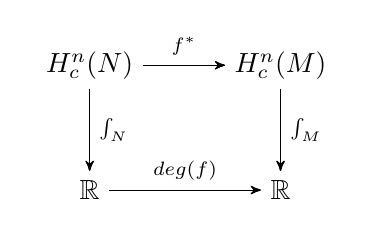
\begin{tikzpicture}
	\matrix (m) [matrix of math nodes, row sep=3em, column sep=3em]
	{  
		\cohomologiacompac{n}{N} & \cohomologiacompac{n}{M}
		\\
		\mathbb{R} & \mathbb{R}
		\\
	};
	{ [start chain] 
		\chainin (m-1-1);
		{ [start branch=A] \chainin (m-2-1)
			[join={node[right,labeled] { \int_{N} }}];
		}
		\chainin (m-1-2) [join={node[above,labeled] {f^{*}} }];
		{ [start branch=A] \chainin (m-2-2)
			[join={node[right,labeled] { \int_{M} }}];
		}
	}
	{ [start chain] 
		\chainin (m-2-1);
		\chainin (m-2-2) [join={node[above,labeled] {deg(f)}}];
	}
	\end{tikzpicture}
	
	Ou seja, $deg(f) \circ \int_{N} = \int_{M} \circ  f^{*} : \cohomologiacompac{n}{N} \to \mathbb{R}$ de modo que
	$$
	\int_{M} f^{*}(\omega) = deg(f) \int_{N} \omega,
	$$
	onde $deg(f) \in \mathbb{R}$ chamado de \textit{grau da aplicação f}.
	
	Note que essa identidade vale para quaisquer $n$-formas a variedade $N$. Além disso, mostraremos um resultado afirmando que, em verdade, $deg(f) \in \mathbb{Z}$, o que é mais impressionante.
	
	\vspace{2mm}
	\textbf{Definição (valor regular e ponto crítico):} Seja $f: M \to N$ uma aplicação suave entre variedades diferenciaveis, dizemos que $p \in M$ é um 
	\textit{ponto crítico} se se $D_{p}f : T_{p}M \to T_{f(p)}N$ for identicamente nula, isto é se $D_{p}f = 0$. Caso o diferencial $D_{p}f : T_{p}M \to T_{f(p)}N$ seja sobrejetor, diremos que esse ponto é um \textit{ponto regular}. Diremos que $f(p) \in N$ é um \textit{valor regular} $\forall q \in f^{-1}(\{p\})$ forem pontos regulares.
	
	Enunciaremos agora alguns teoremas cuja demonstração esta fora do escopo dessa escrita.
	
	\vspace{2mm}
	\textit{\textbf{Teorema (Brower-Sard):} Seja $f: M \to N$ uma aplicação suave entre variedades diferenciaveis, então o conjunto dos valores regulares é um conjunto denso em $N$.}
	
	\vspace{2mm}
	\textit{\textbf{Teorema (Sard) (conjunto de pontos crítico possuem medida nula):} Seja $f: U \subset \mathbb{R}^{n} \to \mathbb{R}^{m}$ uma aplicação suave e definindo $S = \{x \in U: posto(D_{x}f) < m\}$, então o conjunto $f(S)$ é um conjunto de medida (Lebesgue) nula em $\mathbb{R}^{m}$. (Notem que nas condição em que $p \in M$ seja um ponto crítico, teremos $D_{p}f = 0$, logo $posto (D_{p}f) = 0$)}
	
	\vspace{2mm}
	\textit{\textbf{Lema (característica dos pontos regulares em variedades compactas):} $f: M^{n} \to N^{n}$ uma aplicação suave entre variedades diferenciaveis, com mesma dimensão e $M$ compacta. Suponha que $f(p) = q \in N$ seja um valor regular, então $f^{-1}(\{q\}) \subset M$ é um conjunto finito de pontos isolados. Além disso, existe uma vizinhança aberta $U$ de $q$ e abertos disjuntos $V_{i} \ni p_{i}$, onde $p_{i} \in f^{-1}(\{q\})$ são pontos regulares e $1 \leq i \leq k$ tal que}
	\begin{enumerate}
		\item $f^{-1}(U) = \bigcup \limits_{i=1}^{k} V_{i}$
		
		\item $f_{i}:V_{i} \to V$ \textit{é um difeomorfismo para} $1 \leq i \leq k$
	\end{enumerate}
	
	$\square$ Como para todo $p \in f^{-1}(\{q\})$ temos que $D_{p}f : T_{p}M \to T_{f(p)}N$ é sobrejetor, isto é  $posto(D_{p}f) = n$. Sejam $\{\alpha_{j}\}_{j=i}^{n}$ e $\{\beta_{j}\}_{j=i}^{n}$ bases de $T_{p}M$ e $T_{f(p)}N$, respectivamente. Pela sobrejeção do diferencial podemos afirmar que existe ao menos um $\alpha_{j}$ tal que $\beta_{k} = D_{p}f(\alpha_{j})$. Supondo existam $\alpha_{j} \neq \alpha_{k} \in \{\alpha_{j}\}_{j=i}^{n}$ tal que $D_{p}f(\alpha_{j})= D_{p}f(\alpha_{k})$, consequentemente teríamos no máximo $n-1$ elementos para a base de $T_{f(p)}N$, ou seja $posto(D_{p}f) \leq n-1$, o que é uma contradição, pois $posto(D_{p}f) = n$, logo o diferencial é uma aplicação injetora, portanto, é um isomorfismo. Sendo assim, pelo teorema da função inversa, existe uma vizinhança aberta $U \ni p$ difeomorfa a uma vizinhança aberta $Z \ni q$. Consequentemente, tomando $p_{i} \neq p_{j} \in f^{-1}(\{q\})$, teremos $U_{i} \ni p_{i}$ e $U_{j} \ni p_{j}$ difeomorfas as vizinhanças $Z_{i} \ni q$ e $Z_{j} \ni q$, respectivamente, e de modo que ainda tenhamos $U_{i} \cap U_{j} = \emptyset$, isto é, $p_{i} \neq p_{j} \in f^{-1}(\{q\})$ são pontos isolados. Suponha que não o sejam, então para a vizinhança aberta $U_{i} \ni p_{i}$ teremos infinitos outros pontos $p' \in U_{i}$ tais que $f(p') = q$, consequentemente, $D_{p_{i}}f : T_{p_{i}}M \to T_{q}N$ não será injetora, contradizendo o fato afirmado pelo teorema da função inversa demonstrado. Suponha $f^{-1}(\{q\})$ seja infinito, então definindo os fechados $\overline{W_{i}} \subset U_{i}$ tal que $p_{i} \in \overline{W_{i}}$, onde $U_{i}$ são os abertos disjuntos construidos anteriormente. Note que o conjunto $A = \{M \backslash \overline{W_{i}} \} \cup \{U_{i}\}$ definie uma cobertura por abertos de $M$, e como $M$ é compacta, então podemos escolher uma subcobertura finita $A' \subset A$, como $f^{-1}(\{q\})$ é infinito, existirá um $U_{s} \in A'$ contendo infinitos pontos de $f^{-1}(\{q\})$, o que é uma contradição, pois cada aberto $U_{j}$ contém apenas um ponto $p_{j} \in f^{-1}(\{q\})$, portanto $f^{-1}(\{q\})$ é finito. Seja $f^{-1}(\{q\}) = \{p_{1}, \dots, p_{k}\}$ para algum $k \in \mathbb{N}$. Tomemos os abertos $U_{i} \in A'$ da subcobertura finita, e mostramos anteriormente que $f|_{U_{i}} : U_{i} \to f(U_{i}) \subseteq V_{i}$ são difeomorfismos, então $f(U_{i})$ são abertos e $\bigcap(f(U_{i})) \subset N$ é um aberto pois é a intersecção finita de abertos, consequentemente, o conjunto $U^{c} = M \backslash \bigcup U_{i}$ é compacto pois é um subconjunto fechado do compacto $M$, logo $f(U^{c}) \subset N$ é um compacto. Enfim, vamos definir $U = \bigcap f(U_{i}) \backslash f(U^{c})$, e notemos que o conjunto $\bigcap f(U_{i})$ sendo um aberto, todos os seus pontos são interiores, assim, ao se retirar os pontos da intersecção de $f(U^{c})$ com $\bigcap f(U_{i})$ teremos que todos os pontos restantes ainda serão pontos interiores, logo $U =f(U_{i}) \backslash f(U^{c})$ será um conjunto onde todos os pontos são interiores, portanto $U$ é um aberto contendo $q$ o valor regular. Por fim, definindo $V_{i} = U_{i} \cap f^{-1}(U)$ teremos $f^{-1}(U) = \bigcup V_{i}$, como desejávamos. 
	
	$\blacksquare$
	
	\vspace{2mm}
	\textbf{Definição (índice local):} Seja $f : M^{n} \to N^{n}$ uma aplicação suave entre variedades diferenciáveis, compactas  e orientáveis, onde $N$ é conexa. Seja $f(p) = q \in N$ uma valor regular e $p \in f^{-1}(q)$, definimos por \textit{índice local}
	$$
	Ind(f; p) := \left\{
	\begin{array}{cc}
	1, & D_{p}f : T_{p}M \to T_{q}N \text{ preserva orient.} \\
	-1, & \text{caso contrario}.\\
	\end{array}.
	\right.
	$$
	
	\vspace{2mm}
	\textit{\textbf{Teorema (grau de aplicação é um inteiro)} Seja $f : M^{n} \to N^{n}$ uma aplicação suave entre variedades diferenciáveis, compactas e orientáveis, onde $N$ é conexa. Seja $f(p) = q \in N$ uma valor regular e $p \in f^{-1}(\{q\})$, então}
	$$
	deg(f) = \sum \limits_{p \in f^{-1}(q)} Ind(f;p) \in \mathbb{Z}.
	$$
	$\square$ Sejam os pontos regulares $p_{i} \in f^{-1}(\{q\})$ e suas vizinhanças abertas $U_{i} \ni p_{i}$ para $1\leq i \leq k$, sendo $U_{i}$ e o aberto $U \ni q$ definidos como no lema anterior. Seja $\omega \in \Omega^{n}(N)$ tal que $supp(\omega) \subseteq U$, e como $N$ é orientável, podemos supor que $\int_{N} \omega = 1$, então teremos $supp(f^{*}(\omega)) \subseteq f^{-1}(U) = \bigcup V_{i}$, o que nos permite escrever $f^{*}(\omega) = \sum \omega_{i}$, onde $\omega_{i} \in \Omega^{n}(M)$ e $supp(\omega_{i}) \subseteq V_{i}$. Note que teremos $\omega_{i}|_{V_{i}}  = (f|_{V_{i}})^{*}(\omega|_{U})$. Assim:
	$$
	\begin{aligned}
	deg(f) =& deg(f)\int_{N} \omega = \int_{M} f^{*}(\omega)
	\\
	=& \sum \int_{M}\omega_{i} = \sum \int_{V_{i}}\omega_{i}|_{V_{i}}
	\\
	=& \sum \int_{V_{i}} (f|_{V_{i}})^{*}(\omega|_{U}) = \sum Ind(f, p_{i}) \int_{f(V_{i})} \omega|_{U}
	\\
	=& \sum Ind(f, p_{i}) \int_{U} \omega|_{U} = \sum Ind(f, p_{i}) \int_{N} \omega
	\\
	=& \sum Ind(f, p_{i}) \in \mathbb{Z}.
	\end{aligned}$$
	$\blacksquare$
	
	\section{Funções de Morse}
	
	\textbf{Definição (ponto não-degenerado, função de Morse e matriz hessiana):} Sejam $M, N$ variedades diferenciáveis e $f: M \to N$ uma aplicação suave, então dizemos que um ponto $p \in M$ é um \textit{um ponto não-degenerado} a matriz $$
	(D_{p}^{2}f) = \Big( \frac{\partial^{2}f}{\partial x_{i} \partial x_{j}} (p) \Big)
	$$
	for não-singular, isto é, $det(	(D_{p}^{2}f)) \neq 0$. No caso em que $f: M \to \mathbb{R}$, diremos que é uma \textit{função de Morse} se não contém pontos críticos não-degenerados. Além disso, a matriz das derivadas de segunda ordem definidas anteriormente é chamada \textit{matriz hessiana de f}.
	
	\vspace{2mm}
	\textit{\textbf{Teorema (existência de funções de Morse):} Seja $M \subseteq \mathbb{R}^{n+k}$ uma n-variedade diferenciável compacta, e defina $f:M \to \mathbb{R}$ tal que $f(p) = 1/2||p-q||$, para um dado $q \in \mathbb{R}^{n+k}$, então $f$ é uma função de Morse.}
	
	$\square$ Seja $(U,h)$ uma carta de $M$ e $Y_{j}:\mathbb{R}^{n} \to \mathbb{R}^{n+k}$ com $1 \leq j \leq k$ tais que $[Y_{1}(x), \dots, Y_{k}(x)] = T_{h(x)}M^{\perp}$. Como $M$ é compacta, teremos um número finito de cartas, portanto, basta demonstrarmos que a afirmação vale para uma carta arbitrária, e como temos um número finito, a afirmação será aplicaca em um número de cartas que cobrem $M$. Evidentemente teremos $T_{h(x)}\mathbb{R}^{n+k} = T_{h(x)}M^{\perp} \oplus T_{h(x)}M \cong \mathbb{R}^{n+k}$. Definindo $g:\mathbb{R}^{n+k} \to \mathbb{R}^{n+k}$ tal que
	$$
	g(x, y) = h(x) + \sum_{j=1}^{k} y_{j}Y_{j}(x),
	$$
	veremos que a composição $k = f \circ h : \mathbb{R}^{n} \to \mathbb{R}$ resultará em $k(x) =1/2||h(x) - q|| = 1/2 \langle h(x) - q,h(x) - q \rangle $ e a diferencial dessa função será $D_{h(x)}k(v) = \langle h(x) - q, v\rangle$, onde $v = \sum v_{j}\partial_{j}h(x) \in T_{h(x)}M$, o que nos permite afirmar que $ \langle \partial_{j}h(x), Y_{i} \rangle = 0$, por construção, consequentemente, diferenciando essa ultima identidade, teremos $\langle \partial^{2}_{j,m}h(x), Y_{i} \rangle = -\langle \partial_{j}h(x), \partial_{m}Y_{i} \rangle$. Com isso, temos as derivadas parciais
	$$
	\partial_{i}k(v) = \langle h(x) - q, \partial_{i}h(x) \rangle,
	$$
	e consequentemente, as derivadas de segunda ordem
	$$
	\partial_{i,m}g(v) = \langle \partial_{m}h(x), \partial_{i}h(x) \rangle + \langle h(x) - q, \partial^{2}_{i,m}h(x) \rangle.
	$$
	Como $M$ é compacta e $k: M \to \mathbb{R}$ é uma função contínua, então $k(M) \subset \mathbb{R}$ é um compacto, isto é, fechado e limitado, logo possui um máximo e mínimo, consequentemente, existe $p \in M$ tal que $D_{p}k(v) = \langle grad(k), v \rangle = 0$. Suponda que tenhamos uma carta tal que $p \in h(U)$, assim, $D_{p}k(v) = \langle h(x) - q, v \rangle = 0 \Rightarrow h(x) - q \in T_{p}M^{\perp}$. Diferenciando novamente a função $k$:
	$$
	\begin{aligned}
	\frac{\partial^{2}k}{\partial x_{i}\partial x_{j}}(p) =& \langle \partial_{i}h(p), \partial_{j}h(p) \rangle + \langle \underbrace{ h(p) - q }_{\in T_{p}M^{\perp}}, \frac{\partial^{2} h}{\partial x_{i}\partial x_{j}}(p)\rangle
	\\
	=& \langle \partial_{i}h(p), \partial_{j}h(p) \rangle + \langle \sum_{s=1}^{k}a_{s}Y_{s}(p), \frac{\partial^{2} h}{\partial x_{i}\partial x_{j}}(p)\rangle
	\\
	=& \langle \partial_{i}h(p), \partial_{j}h(p) \rangle + \sum_{s=1}^{k}a_{s} \langle Y_{s}(p), \frac{\partial^{2} h}{\partial x_{i}\partial x_{j}}(p)\rangle
	\\
	=& \langle \partial_{i}h(p), \partial_{j}h(p) \rangle - \sum_{s=1}^{k}a_{s} \langle \partial_{j}Y_{s} , \partial_{i}h(p)\rangle
	\\
	=& \langle \partial_{i}h(p), \underbrace{ \partial_{j}h(p) - \sum_{s=1}^{k}a_{s} \partial_{j}Y_{s} }_{\notin T_{p}M^{\perp}} \rangle
	\\
	\neq & 0.
	\end{aligned}
	$$
	Mostramos que a matriz hessiana de $k$ não é identicamente nula. Agora resta-nos mostrar que ela é invertível.
	
	$\blacksquare$
	
	\vspace{2mm}
	\textit{\textbf{Teorema (aproximação quadráticas de funções em variedades):} Seja $p \in M^{n}$ um ponto crítico não-degenerado de $f \in C^{\infty}(M, \mathbb{R})$, então existe uma carta $(U, h)$ de $M$ contendo a origem tal que $p = h(0)$ e 
		$$
		(f \circ h) (q) = f(p) + \sum_{i=1}^{n}\delta_{i}x_{i}^{2}, \; q \in U
		$$
		onde $\delta_{i} \in \{-1,1\}, \; 1\leq j \leq n$.}
	
	$\square$ A demonstração está fora do escopo.	
	
	$\blacksquare$
	
	\vspace{2mm}
	\textbf{Definição (campo vetorial tipo gradiente e índices de Morse ddo ponto crítico):} Seja $f \in C^{\infty}(M, \mathbb{R})$ uma função de Morse, um campo vetorial $X : M \to T_{p}M$ é dito \textit{tipo gradiente de f} se:
	\begin{enumerate}
		\item Para todo ponto não-crítico $p \in M$ tem-se 	
		$D_{p}f(X(p)) > 0$,
		
		\item Se $p \in M^{n}$ é um ponto crítico não-degenerado de $f$, então existe uma carta $(U, h)$ de $M$ contendo a origem tal que $p = h(0)$ tal que
		$$
		(f \circ h) (q) = f(p) - x_{1}^{2} - \dots - x_{\lambda}^{2} + x_{\lambda + 1}^{2} + \dots + x_{n}^{2}, \; q \in U.
		$$ 
		
		\item O índice $\lambda$ damos o nome de \textit{índice de Morse do ponto crítico $p \in M$}
	\end{enumerate}
	
	\vspace{2mm}
	\textit{\textbf{Lema (campos do tipo gradiente para funçoes de Morse):} Toda função de Morse em $M$ admite um campo do tipo gradiente.}
	
	$\square$ Seja $f : M \to \mathbb{R}$ uma função de Morse. Como $M$ é compacta, todo atlas terá um subatlas finito, além disso, vimos em um teorema anterior que todos os pontos críticos de $f$ são isolados, assim podemos construir um atlas $\{U_{i}, h_{i}\}_{i \in K}$, onde $K \subset \mathbb{N}$ é um conjunto finito, tal que, cada ponto crítico não-degenerado $p_{i} \in h_{i}(U_{i})$ e não pertença a outra carta. Seja $\{\phi_{i}\}_{i \in K}$ uma partição da unidade subordinada ao atlas $\{U_{i}, h_{i}\}_{i \in K}$ e tomemos os campos vetoriais $X_{i} = Dh_{i}(grad(f \circ h_{i}))$ e definindo o campo suave em $M$ por $X = \sum \phi_{i} X_{i}$. Suponha que $p \in M$ e $p \notin \{p_{i}\}_{i \in K}$, claro que existe $U_{s}$ tal que $p \in U_{s}$, então 
	$$
	\begin{aligned}
	D_{p}f(X(p)) =& D_{p}f \Big(\underbrace{ \sum \phi_{i}(p) X_{i}(p) }_{p \in U_{s}}\Big) 
	\\
	=& D_{p}f(X_{s}(p)) 
	\\
	=& (D_{p}f \circ Dh_{i})(grad(f \circ h_{i}))
	\\
	=& D(f \circ h_{i})(grad(f \circ h_{i})) 
	\\
	=& \langle grad(f \circ h_{i}), grad(f \circ h_{i}) \rangle 
	\\
	>&0.
	\end{aligned}
	$$
	Portanto, temos o campo $X$ satisfazendo a primeidas das condições. Por fim, supondo agora $p = p_{s} \in \{p_{i}\}$, então teremos, pelo teorema de aproximação quadrática de funções, que existe uma carta $(U, h)$ contendo a origem de modo que $p_{s} = h(0)$ e $(f \circ h) (q) = f(p) + \sum_{i=1}^{n}\delta_{i}x_{i}^{2}, \; x_{i} \in h^{-1}(U), q \in h(U)$. Podemos realizar uma nova parametrização do aberto $W_{s}$ de modo que as coordenada contendo os índices $\delta_{i} = -1$ fiquem ordenadas, isto é, uma nova carta contendo a origem $(W, g)$ que realiza a permuta das componentes, assim:
	$$
	(f \circ g) (q) = f(p) - y_{1}^{2} - \dots - y_{\lambda}^{2} + y_{\lambda+1}^{2} + \dots + y_{n}^{2}, \; q \in W.
	$$
	
	$\blacksquare$
	
	\vspace{2mm}
	\textit{\textbf{Lema:} Seja $f \in C^{\infty}(M, \mathbb{R})$ uma função de Morse e $X \in \mathfrak{X}(M)$ um campo vetorial suave tal que $D_{p}f(X(p)) > 0$ para todo $p \in M$ que não é um ponto crítico de $f$. Seja $p_{0}$ um ponto crítico de $f$ com índice $\lambda$, e se $X(p_{0}) = 0$, então}
	$$
	i(X, p_{0}) = (-1)^{\lambda}.
	$$
	
	$\square$ Sabemos que toda variedade diferenciável admite um campo vetorial do tipo gradiente, então seja $Y =  grad(f)/2 \in \mathfrak{X}(M)$ e tomemos $(U, h)$ como sendo uma carta de $M$ tal que podemos escrever $(f \circ h) (q) = f(p) - y_{1}^{2} - \dots - y_{\lambda}^{2} + y_{\lambda+1}^{2} + \dots + y_{n}^{2}, \; q \in U$. Teremos $(Y \circ h)(q) = grad(f\circ h)(q)/2 = (-y_{1}, \dots, -y_{\lambda}, y_{\lambda+1}, \dots, y_{n})$. Por definição temos $i(Y, p_{0}) = deg(G(Y))$, onde $G(Y) = Y/||Y||$ é o mapa de Gauss associado ao campo $Y$, assim, temos que $G(Y):M \to \mathbb{R}^n$, logo, tomando $\omega  = dx_{1} \wedge \dots \wedge dx_{n} \in \Omega^{n}(\mathbb{R}^{n})$ teremos 
	$$
	\int_{M} G(Y)^{*}(\omega) = \int_{\mathbb{R}^{n}} det(D(G(Y))) \omega = \int_{\mathbb{R}^{n}} (-1)^{\lambda} \omega =    deg(G(Y))\int_{\mathbb{R}^{n}} \omega, 
	$$
	logo $i(Y, p_{0}) = deg(G(Y)) = (-1)^{\lambda}$. Por hipótese temos que existe um campo vetorial $X \in \mathfrak{X}(M)$ do tipo gradiente, isto é, $grad(X(p)) > 0$ e já vimos que $D_{p}f(Y(p)) = D_{p}f(grad(f \circ h)/2) = 1/4\langle grad(f\circ h), grad(f\circ h) \rangle>0$, onde $p \in h(U)\backslash\{p_{0}\}$. Com essas duas ultimas desigualdades podemos afirmar que ambos $X, Y \in \mathbb{R}_{+}$, que é um subconjunto simplesmente conexo, logo podemos definir a homotopia $g: h(U)\backslash\{p_{0}\} \times [0,1] \to \mathbb{R}^{n}\backslash \{0\}$ tal que $g(p, t) = (1-t)X(p) - tY(p)$, e como os índices locais dos campos vetoriais são invariantes por homotopias, temos $i(X, p_{0}) = i(Y, p_{0}) = (-1)^{\lambda}$, como desejávamos.
	
	$\blacksquare$
	
	\vspace{2mm}
	\textit{\textbf{Teorema (índice total de campos):} Seja $M^{n}$ uma variedade diferenciável compacta e $X \in \mathfrak{X}(M)$ com singularidades isoladas. Seja $f \in C^{\infty}(M, \mathbb{R})$ uma função de Morse e $c_{\lambda}$ o número de pontos críticos com índice $\lambda$, então temos:}
	$$
	Index(X) = \sum_{\lambda = 0}^{n}(-1)^{\lambda}c_{\lambda}.
	$$
	
	$\square$ Seja $X \in \mathfrak{X}(M)$ um campo vetorial com pontos críticos isolados, e como $M$ é compacta, então o campo $X$ terá um número fínito de pontos críticos isolados, logo, pela definição de índice total temos $Index(X) = \sum_{i=1}^{k} i(X;p_{i})$, onde $p_{i} \in M$ são os pontos críticos. Pelo resultado do lema anterior, temos
	$$
	Index(X) = \sum_{i=1}^{k} i(X;p_{i}) = \sum_{i=1}^{k} (-1)^{\lambda_{i}} = \sum_{\lambda}(-1)^{\lambda}c_{\lambda},
	$$
	como desejávamos.
	
	$\blacksquare$
	
	\section{Teoria de Morse - Alguns Resultados}
	
	\textit{\textbf{Lema (particionamento da característica de Euler-Poincaré):} Sejam $M$ uma variedade diferenciável e $U, V \subset M$ abertos tais que $M = U \cup V$ e $U \cap V$ tenha cohomologia com dimensão finita, então:}
	$$
	\chi(U \cup V) = \chi(U) + \chi(V) - \chi(U \cap V).
	$$
	
	$\square$ Aplicando a sequência de Mayer-Vietoris, teremos
	$$
	\dots \to H^{p}(U \cup V) \to H^{p}(U) \oplus H^{p}(V) \to H^{p}(U  \cap V) \to H^{p+1}(U \cup V) \to \dots
	$$
	
	$\blacksquare$
	
	\vspace{2mm}
	\textbf{Definição (nível de variedade segundo função de Morse):} Sejam $M^{n}$ uma variedade diferenciável, $f \in C^{\infty}(M, \mathbb{R})$ uma função de Morse e tome $a \in \mathbb{R}$, então definimos o conjunto
	$$
	M(a) = \{p \in M: f(p) <a \}.
	$$
	
	\textit{\textbf{Lema (níveis difeomorfos):} Se não existirem pontos críticos no intervalo $[a, b]$, então os conjuntos $M(a)$ e $M(b)$ são difeomorfos.}
	
	$\square$ Demonstração esta fora do escopo.
	
	$\blacksquare$
	
	\vspace{2mm}
	\textit{\textbf{Lema (níveis difeomorfos):} Seja $a \in \mathbb{R}$ um valor crítico de $f:M \to \mathbb{R}$, e suponha que $\{p_{i}\} \subset f^{-1}(\{a\})$, $1\leq i \leq k$ o conjunto de pontos críticos com índices $\lambda_{i}$, então existe $\epsilon > 0 \in \mathbb{R}$ e uma união disjunta de abertos $U_{i} \ni p_{i}$ tais que:}
	\begin{enumerate}
		\item  \textit{os pontos $\{p_{i}\}$ são os únicos pontos críticos no conjunto $f^{-1}([a - \epsilon, a + \epsilon])$.}
		
		\item \textit{cada $U_{i}$ é difeomorfo a um aberto contrátil de $\mathbb{R}^{n}$.}
		
		\item \textit{$W_{i} := U_{i} \cap M(a-\epsilon)$ é difeomorfo a $S^{\lambda_{i} - 1} \times V_{i}$, onde $V_{i} \subset \mathbb{R}^{n - (\lambda_{i} - 1)}$ é um aberto contrátil.}
		
		\item \textit{$M(a+\epsilon)$ é difeomorfo a $U_{1} \cup \dots \cup U_{k} \cup M(a-\epsilon)$.}
	\end{enumerate}
	
	$\square$ Demonstração esta fora do escopo.
	
	$\blacksquare$
	
	\section{Teorema Poicaré-Hopf}
	
	\vspace{2mm}
	\textit{\textbf{Proposição (característica de Euler-Poincaré e índices de Morse):} Assumindo as hipóteses do lema anterior, e supondo que a variedade $M^{n}$ possua toa a sua cohomologia com dimensão finita, então:}
	$$
	\chi(M(a+\epsilon)) = \chi(M(a-\epsilon)) + \sum_{\lambda}(-1)^{\lambda}c_{\lambda}.
	$$
	
	$\square$ Como cada aberto $U_{i}$ é contrátil, então seus grupos de cohomologia são isomorfos aos grupos de cohomologia do ponto, isto é, $H^{p}(U_{i})  = \{[0]\}$ se $p > 0$ e $H^{0}(U_{i}) \cong \mathbb{R}$, logo, $U = U_{1} \cup \dots \cup U_{k}$, que é uma união disjunta de abertos, tem como grupo de cohomologia a seguinte soma direta $H^{0}(U) = H^{0}(U_{1}) \oplus \dots \oplus H^{0}(U_{k}) \cong \mathbb{R} \oplus \dots \oplus \mathbb{R} \cong \mathbb{R}^{k}$, por fim, $H^{p}(U) = \{[0]\}$. Sabemos que $U_{i} \cap M(a-\epsilon) \cong S^{\lambda_{i} - 1} \times V_{i}$, e que $V_{i}$ é contrátil, logo, possui a mesma homotopia de um ponto, portanto $S^{\lambda_{i} - 1} \times V_{i}$ possui a mesma homotopia de $S^{\lambda_{i} - 1} \times \{q\}$, para algum $q \in V_{i}$, consequentemente, $H^{p}(W_{i}) = H^{p}(S^{\lambda_{i} - 1} \times V_{i}) \cong H^{p}(S^{\lambda_{i} - 1} \times \{q\}) \cong H^{p}(S^{\lambda_{i} - 1})$, onde já vimos que $H^{p}(S^{\lambda_{i} - 1}) \cong \mathbb{R}$ para $p \in \{0, \lambda_{i} - 1\}$ e $H^{p}(S^{\lambda_{i} - 1}) = \{[0]\}$ para $p \notin \{0, \lambda_{i} - 1\}$. Como $U_{i}$ são disjuntos, então $W_{i} = U_{i}\cap M(a-\epsilon)$ são dois a dois disjuntos, logo $U \cap M(a-\epsilon) = W_{1} \cup \dots \cup W_{k}$ é uma união disjunta, consequentemente, $H^{p}(U \cap M(a-\epsilon)) = H^{p}(W_{1}) \oplus \dots \oplus H^{p}(W_{k}) \cong \mathbb{R}^{k}$, para $p \in \{0, \lambda_{i} - 1\}$ e $H^{p}(U \cap M(a-\epsilon)) \cong \{[0]\}$ para $p \notin \{0, \lambda_{i} - 1\}$. Aplicando o lema anterior que escreve a característica de Euler em uma sequência de Mayer-Vietoris para o particionamento do conjunto $M(a+\epsilon) = U \cup M(a-\epsilon)$, teremos $\chi(M(a+\epsilon)) = \chi(U) + \chi(M(a-\epsilon)) - \chi(U \cap M(a-\epsilon))$, mas vimos que 
	$$
	\begin{aligned}
	\chi(U) =& \sum (-1)^{i}dim(H^{i}(U)) = dim(H^{0}(U)) = k
	\\
	\chi(U \cap M(a-\epsilon)) =& \sum (-1)^{i}dim(H^{i}(U \cap M(a-\epsilon))) 
	\\
	=& dim(H^{0}(U \cap M(a-\epsilon))) + \sum_{i}(-1)^{\lambda_{i} - 1} 
	\\
	=& k + \sum_{\lambda}(-1)^{\lambda - 1}c_{\lambda} 
	\\
	=& k - \sum_{\lambda}(-1)^{\lambda}c_{\lambda},
	\end{aligned}
	$$
	logo, voltando na igualdade 
	$$
	\begin{aligned}
	\chi(M(a+\epsilon)) =& \chi(U) + \chi(M(a-\epsilon)) - \chi(U \cap M(a-\epsilon))
	\\
	=& k +\chi(M(a-\epsilon)) - k + \sum_{\lambda}(-1)^{\lambda}c_{\lambda}
	\\
	=& \chi(M(a-\epsilon)) + \sum_{\lambda}(-1)^{\lambda}c_{\lambda}.
	\end{aligned}
	$$
	
	$\blacksquare$
	
	\vspace{2mm}
	\textit{\textbf{Teorema (Característica de Euler-Poincaré):} Seja $f \in C^{M, \mathbb{R}}$ uma função de Morse e $M$ uma variedade diferenciável compacta, então:
		$$
		\chi(M^{n}) = \sum_{\lambda}(-1)^{\lambda}c_{\lambda},
		$$
		onde $c_{\lambda}$ é o número de pontos críticos com índice $\lambda$.}
	
	$\square$ Como $M$ é compacta e como $f$ é contínua, logo $f(M) = [a,b] \subset \mathbb{R}$ é um compacto e $f$ possui um número finito de pontos críticos. Sejam  os valores críticos não-degenerados $\{f(p_{i})\}_{1\leq i \leq k}$ e, sem perda de generalidade, podemos supor que $a_{1} = f(p_{1}) < \dots < a_{k}=f(p_{k})$. Tomemos $b_{0} < a_{1}$, $a_{k} < b_{k}$ e $b_{i} \in (a_{i}, a_{i+1})$ onde $1\leq i \leq k-1$. Note que $(a_{i}, a_{i+1})$ não possui valores críticos, então pelo lema dos níveis difeomorfos temos $M(b_{i}) \simeq M(c_{i}), \; \forall b_{i}, c_{i} \in (a_{i}, a_{i+1})$. Tomemos $\{b_{i}\}_{0\leq i \leq k}$ arbitrários, mas fixos, assim, pela proposição anterior para cada valor regular não-degenerados $a_{i} \in [b_{i}, b_{i+1}]$, existe um $\epsilon_{j} > \mathbb{R}$ tal que
	$$
	\chi(M(a_{i} + \epsilon_{i})) = \chi(M(a_{i}-\epsilon_{i})) + \sum_{\lambda}(-1)^{\lambda}c_{\lambda}.
	$$
	Como $a_{i} \in [b_{i}, b_{i+1}]$ é o unico valor regular nesse intervalo, podemos tomar $\epsilon_{i} = b_{i} - a_{i}$, de modo que teremos $\chi(M(a_{i} + \epsilon_{i})) = \chi(M(a_{i} + b_{i} - a_{i})) = \chi(M(b_{i}))$, por outro lado, temos que $M(a_{i} - \epsilon_{i}) \simeq M(b_{i-1})$ pois o intervalo $[b_{i-1}, a_{i} - \epsilon_{i})$ não contém valores regulares, portanto temos
	$$
	\chi(M(b_{i})) = \chi(M(b_{i-1})) + \sum_{\lambda_{i}}(-1)^{\lambda_{i}}c_{\lambda_{i}}.
	$$
	Por definição temos que $M(b_{0}) = \emptyset$ e $M(b_{k}) = M$, consequentemente, $\chi(M(b_{0}))=0$ e $\chi(M(b_{k}))=\chi(M)$. Reescrevendo a relação anterior como
	$$
	\sum_{p \in f^{-1}(\{a_{i}\})}(-1)^{\lambda_{p}} = 	\chi(M(b_{i})) - \chi(M(b_{i-1})),
	$$
	devemos percorrer todos os valores regulares, isto é, somando todas suas contribuições para a característica de Euler-Poincaré, assim:
	$$
	\begin{aligned}
	\sum_{i=1}^{k} \Big(\sum_{p \in f^{-1}(\{a_{i}\})}(-1)^{\lambda_{p}}\Big) =& 		\sum_{i=1}^{k} \Big(\chi(M(b_{i})) - \chi(M(b_{i-1}))\Big)
	\\ 
	=&  \chi(M(b_{1})) - \chi(M(b_{0}) + \chi(M(b_{2})) - \chi(M(b_{1}) + \dots + \chi(M(b_{k}))
	\\
	=& \chi(M(b_{k})) 
	\\
	=& \chi(M),
	\end{aligned}$$
	pois tivemos cancelamentos alternados nas somas das características. Por fim, reescrevendo
	$$
	\chi(M)	= \sum_{i=1}^{k} \Big(\sum_{p \in f^{-1}(\{a_{i}\})}(-1)^{\lambda_{p}}\Big) = \sum_{i=1}^{m}(-1)^{\lambda_{i}} = \sum_{\lambda}(-1)^{\lambda}c_{\lambda}.
	$$
	
	$\blacksquare$
	
	\vspace{2mm}
	\textit{\textbf{Teorema de Gauss-Bonnet (para superfícies em $\mathbb{R}^{3}$)}: Seja $S^{2} \subset \mathbb{R}^{3}$ uma variedade compacta, orientável de dimensão 2, (isto é, uma superfície regular e compacta e orientável). Definindo $K:S \to \mathbb{R}$ como a curvatura Gaussiana de $S$, então:}
	$$
	\int_{S} K vol_{S} = 2\pi \chi(S).
	$$
	
	$\square$ Seja $N : S \to S^{2}$ o mapa de Gauss da superfície $S$, logo $D_{p}N :T_{p}S \to T_{N(p)}S^{2} $, e utilizando o resultado já conhecido de teoria das súperfícies regulares, podemos afirmar que $K(p) = det(D_{p}N)$. Vamos rotacionar a superfície $S$ de modo a garantir que os pólos da esféra sejam valores regulares de $N$, isto é, existem $p_{\pm} \in S$ é tal que $N(p_{\pm}) = (0,0,\pm 1) \in S^{2}$ e $D_{p_{\pm}}N \neq 0$. Seja $f : S \to \mathbb{R}$ tal que $f(x,y,z) = z$, como sendo a função que mensura a distancia dos pontos de $S$ para o plano $P = \{(x,y,0) \in \mathbb{R}^{3} \}$. É evidente que essa funções é contínua, e como $S$ é compacta, então $f(S) \subset \mathbb{R}$ é um compacto, portanto e um intervalo fechado, assim $f$ possui um máximo e um mínimo. Calculando o diferencila nesses pontos de extremos teremos:
	$$
	D_{p}f(v) = \langle grad(f), v\rangle = \langle (0,0,1), v\rangle = v_{3}, 
	$$
	logo, $Ker(D_{p}f) = \{(v_{1}(p), v_{2}(p), 0) \in \mathbb{R}^{3} \} = T_{p}S$, pela construção anterior, portanto $D_{p}f(T_{p}S)  = \{0\}$, como afirmado, consequentemente, os pontos críticos são todos aqueles em que o mapa de gauss tem sua imagem em um dos pólos da esféra, ou seja, se $p \in S$ é um ponto de máximo/mínimo, então $N(p) = (0,0,\pm 1)$. Seja $p \in S$ tal que $N(p) = (0,0,\pm 1)$, e como construído, $D_{p}N \neq 0$, logo é um isomorfismo, portanto $K(p) = det(D_{p}N) \neq 0$. Seja $(U, h)$ uma carta de $S$ tal que $p \in h(U)$ e temos a parametrização $h(U) = \{(x(u,v), y(u,v), z(u,v)): (u,v ) \in U \}$, e pelo teorema da função implícita, toda superfície é localmente o gráfico de uma função, o que nos permite escrever escolher uma vizinhança de $p$ tal que, para algum $W \subset U$ temos $V \subset h(U)$ e $V=\{(u, v , z(u,v)): (u,v) \in W\} = \{(u, v , f(u,v)): (u,v) \in W\}$. Temos que a curvatura gaussiana restrita a essa carta poderá ser escrita como:
	$$
	K(p) = \Big\{1+ \Big(\frac{\partial f}{\partial u}(p)\Big)^{2} + \Big(\frac{\partial f}{\partial v}(p)\Big)^{2} \Big\}^{-1} det(D_{p}^{2}f), \; p \in V.
	$$
	E como sabemos que $K(p) = det(D_{p}N) \neq 0 \Rightarrow  det(D_{p}f) \neq 0$, logo, $p \in V$ é um ponto crítico não-degenerado, portanto $f: S \to \mathbb{R}$ é uma função de Morse, e podemos escrever:
	$$
	f \circ h (q) = f (p) + au^{2} + b v^{2}, \; q \in W,  
	$$
	assim, nesse aberto $W$ teremos $\partial^{2}(f\circ h)(q)/\partial u \partial v = 0$, com isso teremos  determinante 
	$$
	det \Big(D_{q}^{2}(f\circ h) \Big) = \frac{\partial^{2}(f\circ h)}{\partial^{2}u}\frac{\partial^{2}(f\circ h)}{\partial^{2}v} = 4ab,
	$$
	logo se $K(q) > 0 \Rightarrow det(D_{q}^{2}f) > 0$, portanto deveremos ter $a = b \in \{1, -1\}$. Caso $a = b = 1$ então teremos um ponto crítico não-degenerado com índice $0$, já no caso em que $a=b=-1$, teremos um ponto crítico não degenerado com índice $2$. Por outro lado, se $K(q) < 0$, teremos $a \neq b $ e $a, b \in \{1, -1\}$, sendo que em quaisquer um dos casos teremos um ponto crítico com índice $1$, apenas. Calculando a caracterísica de Euler-Poicaré $\chi(S) = \sum_{\lambda}(-1)^{\lambda}c_{\lambda}$ para ambos os casos, veremos que no caso $K(q) > 0$
	$$
	\chi(S) = \#\{p \in S: K(p)>0, \; N(p) = (0,0,\pm 1)\},
	$$
	por outro lado, sabemos que $p_{\pm} \in S^{2}$ são valores regulares de $N$, consequentemente, sabemos pelo teorema do índice de campos que
	$$
	deg(N) = \#\{p \in N^{-1}(p_{+} ): K(p)>0 \}
	$$
	e também 
	$$
	deg(N) = \#\{p \in N^{-1}(p_{-} ): K(p)>0 \},
	$$
	logo temos a relação $\chi(S) = 2 deg(N)$. Por fim, sabemos relacionar os $2-$volumes de ambas as superfícies, e é realizada por $N^{*} : \Omega^{2}(S^{2}) \to \Omega^{2}(S)$, tal que $N^{*}(vol_{S^{2}}) = det(D_{p}N)vol_{S} = K(p)vol_{S}$. Integrando ambos os volumes, teremos:
	$$
	\begin{aligned}
	\int_{S}Kvol_{S} =& \int_{S^{2}}N^{*}(vol_{S^{2}}) 
	\\
	=& deg(N) \underbrace{\int_{S^{2}}vol_{S^{2}} }_{= 4\pi}
	\\
	=& 4\pi deg(N)
	\\
	=& 2\pi \chi(S).
	\end{aligned}
	$$
	
	$\blacksquare$
	
	\section{Dualidade de Poincaré}
	
	Quando trabalhamos com integração em variedades não-compactas operacionamos sobre formas com suporte compacto, caso as variedades sejam compactas, então esse caso cobre o anterior. Assim, tomemos $M^{n}$ uma variedade diferenciável e $\omega \in \Omega_{c}^{n}(M)$, e por definição, $\int_{M}\omega \in \mathbb{R}$, isto é, $\int_{M} \in \Omega_{c}^{n}(M)^{*}$ pois é um operador linear, por construção. Como, a partir da operação de integração, construir um funcional linear em $\Omega_{c}^{p}(M)^{*}$ onde $1 \leq p \leq n-1$. Seja $0\leq k \leq n$ e reescreveremos $p = n-k$, sendo que $k=0$ é o caso conhecido. Para cada $k$ tome $\alpha \in \Omega^{k}(M)$ e definindo $D : \Omega^{k}(M) \to \Omega_{c}^{n-k}(M)^{*}$ tal que $D(\alpha)(\omega) = \int_{M}\alpha \wedge \omega \in \mathbb{R}$. Note que através do produto exterior conseguimos um funcional para cada $p = n-k$, podendo integrar na variedade, como desejávamos. Além disso, essa integração essa aplicação bem-definida pois temos $supp(\alpha\wedge \omega) = supp(\alpha) \cap supp(\omega) \subset supp(\omega)$, logo
	$$
	D(\alpha)(\omega) = \int_{M}\alpha \wedge \omega  = \int_{supp(\alpha \wedge \omega  )}\alpha \wedge \omega  \leq \int_{supp(\omega)}\alpha \wedge \omega < \infty,$$
	e como o $supp(\omega)$ é compacto, então o funcional $D(\alpha) \in H^{n-k}_{c}(M)$ esta bem-definido. 
	
	\vspace{2mm}
	\textit{\textbf{Proposição (funcional linear da homologia):} Seja $M^{n}$ uma variedade diferenciável e orientável, então o mapa $D_{M}: H^{k}(M) \to H^{n-k}_{c}(M)^{*}$ dado por $D_{M}([\alpha]) = \int_{M} \alpha \wedge$ esta bem definido e resulta em um funcional linear, sendo que sua operação esta definida como}
	$$
	D_{M}([\alpha])([\omega]) = \Big( \int_{M} \alpha \wedge \Big)([\omega]) = \int_{M} \alpha \wedge \omega.
	$$
	
	$\square$ Tomemos $[\alpha] = [\beta] \in H^{k}(M)$ e um $[\omega] \in H^{n-k}(M)^{*}$, então
	$$
	\begin{aligned}
	D_{M}([\alpha])([\omega]) =& \int_{M} \alpha \wedge \omega = \int_{M} (\beta + d\lambda)\wedge \omega
	\\
	=& \int_{M} \beta \wedge \omega + \int_{M}d\lambda \wedge \omega
	\\
	=& \int_{M} \beta \wedge \omega + \int_{M}d(\lambda \wedge \omega) - (-1)^{k}\lambda \wedge d\omega
	\\
	=&\int_{M} \beta \wedge \omega + \underbrace{ \int_{\partial M}\lambda \wedge \omega }_{=0} + \underbrace{ \int_{M} (-1)^{k+1}\lambda \wedge d\omega }_{=0}
	\\
	=& \Big( \int_{M} \beta \wedge \Big)([\omega])
	\\
	=& D_{M}([\beta])([\omega]),
	\end{aligned}
	$$ 
	onde nas duas passagens anteriores aplicamos o teorema de Stokes e utilizamos o fato de que a variedade não contém bordo, e também o fato de que $\omega$ é fechada pois $[\omega] \in H^{n-k}_{c}(M) \Rightarrow \omega \in Z^{n-k}_{c}(M)$, logo $d\omega=0$. Portanto, esta bem-definido. Sejam $a \in \mathbb{R}$ e $[\beta], [\omega] \in  H^{n-k}_{c}(M)$, então é claro que $a[\beta]+[\omega] \in  H^{n-k}_{c}(M)$ e assim
	$$
	D_{M}([\alpha])(a[\beta]+[\omega] ) = D_{M}([\alpha])([a\beta+\omega]) = \int_{M}\alpha \wedge (a\beta+\omega) = a\int_{M}\alpha \wedge \beta + \int_{M}\alpha \wedge \omega = aD_{M}([\alpha])([\beta]) + D_{M}([\alpha])([\omega] ),
	$$ 
	portanto é linear.
	
	$\blacksquare$
	
	\vspace{2mm}
	\textit{\textbf{Lema (dualidade do $\real{n}$):} A aplicação $D_{\real{n}} : \cohomologia{p}{\real{n}} \to \cohomologiacompacdual{n-p}{\real{n}}$ é um isomorfismo para $0 \leq p \leq n$}.
	
	$\square$ Por construção $D^{\real{n}}$ é uma aplicação linear. Sabemos que a cohomologia é desse espaço dada por $\cohomologia{0}{\real{n}} \cong \real{}$ e $\cohomologia{p}{\real{n}} = 0$ para $p>0$. Primeiramente, notemos que para todo $0\leq p \leq n$ temos a relação de continência $\cohomologiacompac{p}{\real{n}} \subseteq \cohomologia{p}{U}$, e nos casos em que $p>0$ temos $\cohomologia{p}{\real{n}} = 0 \Rightarrow \cohomologiacompac{n-p}{\real{n}} \subseteq \cohomologia{n-p}{\real{n}} = 0$, logo $\cohomologiacompac{n-p}{\real{n}}=0$ e $D_{\real{n}}$ é o isomorfismo trivial $0 \mapsto 0$. Agora nos resta o caso em que $p=0$. Tomando as classes das funções constantes $[a] \in \cohomologia{0}{\real{n}}$ e $[\omega] \in \cohomologiacompac{n}{\real{n}}$ tal que $\int_{\real{n}}\omega = 1$, então $D_{\real{n}}([a])([\omega]) = \int_{\real{n}} a\omega = a\int_{\real{n}} \omega = a \in \real{}$. Podemos ver que é injetora pois $D_{\real{n}}([a])([\omega]) = a = 0 \Rightarrow [a] = [0]$, portanto $Ker(D_{\real{n}}) = \{0\}$, e é sobrejetora pois, dado $b \in \real{}$, podemos tomar um $[b] \in \cohomologia{0}{\real{n}}$ tal que $D_{\real{n}}([b])([\omega]) = b \in \real{}$. Portanto $D_{\real{n}}$ é um isomorfismo para $0\leq p \leq n$, como desejávamos. 
	
	$\blacksquare$
	
	\vspace{2mm}
	\textit{\textbf{Corolário (equivalência entre dualidade do $\real{n}$):} Seja $U \subseteq M^{n}$ um subconjunto de um n-variedade diferenciável e orientável. Se $U$ for homeomorfo a $\real{n}$, então $D_{U} \cong D_{\real{n}}$.}
	
	$\square$ Como $U$ e $\real{n}$ são homeomorfos, então suas cohomologias são isomorfas, então seja $\psi : U \to \real{n}$ esse homeomorfismo e $\psi^{*} : \cohomologia{p}{U} \to \cohomologia{p}{\real{n}}$ o isomorfismo, assim temos o diagrama:
	\\
	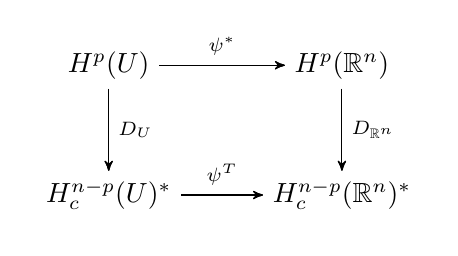
\begin{tikzpicture}
	\matrix (m) [matrix of math nodes, row sep=3em, column sep=3em]
	{  
		H^{p}(U) & H^{p}(\real{n})
		\\
		H^{n - p}_{c}(U)^{*} & H^{n - p}_{c}(\real{n})^{*}
		\\
	};
	{ [start chain] 
		\chainin (m-1-1);
		{ [start branch=A] \chainin (m-2-1)
			[join={node[right,labeled] {D_{U}}}];
		}
		\chainin (m-1-2) [join={node[above,labeled] {\psi^{*}} }];
		{ [start branch=A] \chainin (m-2-2)
			[join={node[right,labeled] { D_{\real{n}} }}];
		}
	}
	{ [start chain] 
		\chainin (m-2-1);
		\chainin (m-2-2) [join={node[above,labeled] {\psi^{T}}}];
	}
	\end{tikzpicture}
	
	Sabemos que dado um espaço vetorial $A$, então $* : A \to A^{*}$ é um isomorfismo, além disso, se $B$ for um espaço vetorial e $\psi : A \to B$ for um isomorfismo, então $\psi^{T} := *\circ \psi \circ *^{-1} : A^{*} \to B^{*}$ é um isomorfismo, poi é a composição de isomorfismos.
	
	Com isso, a aplicação $\Psi^{T}: \cohomologiadual{p}{U} \to \cohomologiadual{p}{\real{n}}$ é um isomorfismo, pois basta fazermos $A = \cohomologia{p}{U}$ e $B = \cohomologia{p}{\real{n}}$, agora definindo o a aplicação do diagrama $\psi^{T} := \Psi^{T}|_{\cohomologiacompacdual{p}{U}}$ para $0\leq p \leq n$, teremos o isomorfismo desejado. Sendo assim, o diagrama comuta, portanto, podemos afirmar que $\psi^{T}\circ D_{U} = D_{\real{n}} \circ \psi^{*} \Rightarrow D_{U} = D_{\real{n}} \circ \psi^{*} \circ (\psi^{T})^{-1}$, logo $D_{U}$ e $D_{\real{n}}$ são equivalentes a menos do isomorfismo $\psi^{*} \circ (\psi^{T})^{-1}$, portanto $D_{U} \cong D_{\real{n}}$, como desejávamos.
	
	$\blacksquare$
	
	\vspace{2mm}
	\textit{\textbf{Teorema (existência da Dualidade de Poincaré):} Seja $M^{n}$ uma n-variedade diferenciável e orientável, então existe $U \subseteq M$ tal que $D_{U} : \cohomologia{p}{U} \to \cohomologiacompacdual{n-p}{U}$ é um isomorfismo para $0 \leq p \leq n$ .}
	
	$\square$ Sabemos que existe ao menos uma carta $(V, h)$ de $M$ tal que $U = h(V) \subseteq M$ é homeomorfo a bola aberta $V \subseteq \real{n}$, consequentemente, $\cohomologia{p}{U} \cong \cohomologia{p}{V}$. Contudo, toda bola aberta $V$ é homeomorfa a $\real{n}$, logo $\cohomologia{p}{U} \cong \cohomologia{p}{\real{n}}$, consequentemente, $D_{U} \cong D_{\real{n}}$, e pelo \textit{lema da dualidade do $\real{n}$}, $D_{\real{n}}$ é um isomorfismo, logo $D_{U}$ é um isomorfismo, como desejávamos.
	
	$\blacksquare$

	\vspace{2mm}
	\textit{\textbf{Lema:} Sejam $M^{n}$ uma variedade e  $V \subseteq U \subset M$ dois abertos, então o diagrama abaixo é comutativo.}
	\\
	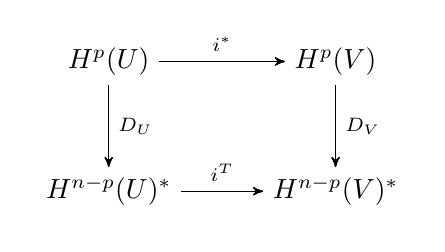
\begin{tikzpicture}
	\matrix (m) [matrix of math nodes, row sep=3em, column sep=3em]
	{  
		H^{p}(U) & H^{p}(V)
		\\
		H^{n - p}(U)^{*} & H^{n - p}(V)^{*}
		\\
	};
	{ [start chain] 
		\chainin (m-1-1);
		{ [start branch=A] \chainin (m-2-1)
			[join={node[right,labeled] {D_{U}}}];
		}
		\chainin (m-1-2) [join={node[above,labeled] {i^{*}} }];
		{ [start branch=A] \chainin (m-2-2)
			[join={node[right,labeled] {D_{V}}}];
		}
	}
	{ [start chain] 
		\chainin (m-2-1);
		\chainin (m-2-2) [join={node[above,labeled] {i^{T}}}];
	}
	\end{tikzpicture}
	
	$\square$ Primeiramente, observemos que dado um cíclo $\omega \in \Omega^{p}(U)$, então teremos que $\omega \in \Omega^{p}(V)$, isto é, $Z^{p}(U) \subseteq Z^{p}(V)$, logo, $H^{p}(U) \subseteq H^{p}(V)$, portanto a aplicação de inclusão do diagrama esta bem-definida.
		
	$$
	\begin{aligned}
	(D_{V}\circ i^{*} )([\beta])([\omega])
	=& D_{V} ([i^{*}(\beta)]) = \Big( \int_{V} i^{*}(\beta) \wedge \Big)([\omega]) = \int_{V} i^{*}(\beta) \wedge \omega = \int_{V} \beta \wedge \omega 
	\\
	(i^{T} \circ D_{U})([\beta])([\omega]) =& i^{T}(D_{U}([\beta]))([\omega]) = i^{T}\Big( \int_{U} \beta \wedge \Big)([\omega]) = \int_{U} \beta|_{V} \wedge i^{*}(\omega),
	\end{aligned}
	$$	
	como $supp_{U}(\beta|_{V} \wedge i^{*}(\omega)) = supp_{V}(\beta|_{V} \wedge \omega) \subseteq  supp_{V}(\beta \wedge \omega) = supp_{V}(\omega)$, logo a ultima integral será
	$$
	(i^{T} \circ D_{U})([\beta])([\omega]) =\int_{U} \beta|_{V} \wedge i^{*}(\omega) = \int_{V} \beta \wedge \omega.
	$$
	
	Como $[\beta] \in H^{p}(U)$ e $[\omega] \in H^{p}_{c}(V)^{*}$ são arbitrários, então $D_{U}\circ i^{*}  = i^{T} \circ D_{U}$, e portanto o diagrama comuta.
	
	$\blacksquare$
	
	\vspace{2mm}
	\textit{\textbf{Proposição (aplicação bordo)}:} Sejam $U, V \subseteq M^{n}$ dois aberto de uma n-variedade diferenciável tais que $M = U \cup V$. Tome a aplicação $\partial^{*}: H^{p}(U\cap V) \to H^{p+1}(M)$, então a aplicação transposta será $\partial^{T} : H^{n-p}(U\cap V)^{*} \to H^{n-p-1}(M)^{*}$ tal que, dado $[\omega] \in H^{p}(U \cap V)$, teremos $\partial^{T}(D_{U\cap V}([\omega])) := D_{M}(\partial^{*}([\omega]))$. Essa aplicação esta bem-definida.
	
	$\square$ Sejam $[\omega] \in H^{p}(U \cap V)$ e $[\gamma] \in H^{n-p-1}_{c}(M)$, teremos:
	$$
	\partial^{T}(D_{U\cap V}([\omega]))([\gamma]) = D_{M}(\partial^{*}[\omega])([\gamma]) = D_{M}([\alpha])([\gamma]) = \int_{M} \alpha \wedge \gamma,
	$$
	onde definimos $[\alpha] = \partial^{*}[\omega] \in H^{p+1}(M)$. Assim, podemos ver que $\alpha \wedge \gamma$ é uma $n$-forma e também a integral existe pois $supp(\alpha \wedge \gamma) \subseteq supp(\alpha) \cap supp(\gamma) \subseteq supp(\gamma)$, logo, 
	$$
	\partial^{T}(D_{U\cap V}([\omega]))([\gamma]) = \int_{M} \alpha \wedge \gamma = \int_{supp(\alpha \wedge \gamma)} \alpha \wedge \gamma \leq \int_{supp(\gamma)} \alpha \wedge \gamma < \infty,
	$$
	logo a aplicação esta bem-definida.
	
	$\blacksquare$
	
	\vspace{2mm}
	\textit{\textbf{Lema (functores entre sequências Mayer-Vietories):} Sejam $M^{n}$ uma variedade e  $U,V \subset M$ dois abertos tais que $M=U \cup V$, então o diagrama abaixo é comutativo.}
	\\
	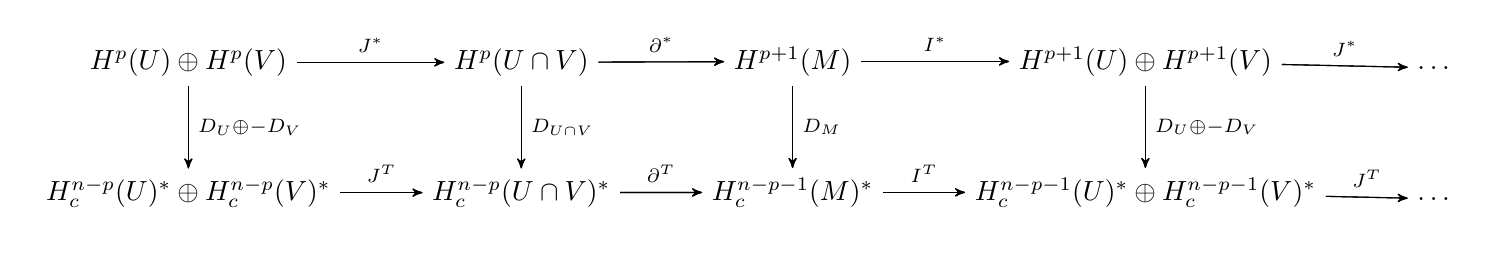
\begin{tikzpicture}
	\matrix (m) [matrix of math nodes, row sep=3em, column sep=3em]
	{  
		H^{p}(U) \oplus H^{p}(V) & H^{p}(U \cap V) & H^{p+1}(M)  & H^{p+1}(U) \oplus H^{p+1}(V) & \dots
		\\
		H^{n - p}_{c}(U)^{*} \oplus H^{n- p}_{c}(V)^{*} & H^{n - p}_{c}(U \cap V)^{*} & H^{n - p-1}_{c}(M)^{*} & H^{n - p-1}_{c}(U)^{*} \oplus H^{n - p-1}_{c}(V)^{*} & \dots
		\\
	};
	{ [start chain] 
		\chainin (m-1-1);
		{ [start branch=A] \chainin (m-2-1)
			[join={node[right,labeled] {D_{U} \oplus -D_{V}}}];
		}
		\chainin (m-1-2) [join={node[above,labeled] {J^{*}} }];
		{ [start branch=A] \chainin (m-2-2)
			[join={node[right,labeled] {D_{U \cap V}}}];
		}
		\chainin (m-1-3) [join={node[above,labeled] {\partial^{*} }}];
		{ [start branch=B] \chainin (m-2-3)
			[join={node[right,labeled] { D_{M} }}];
		}
		\chainin (m-1-4) [join={node[above,labeled] {I^{*}}}];
		{ [start branch=C] \chainin (m-2-4)
			[join={node[right,labeled] { D_{U} \oplus -D_{V} }}];
		}
		\chainin (m-1-5) [join={node[above,labeled] {J^{*}}}];
	}
	{ [start chain] 
		\chainin (m-2-1);
		\chainin (m-2-2) [join={node[above,labeled] {J^{T}}}];
		\chainin (m-2-3) [join={node[above,labeled] {\partial^{T} }}];
		\chainin (m-2-4) [join={node[above,labeled] {I^{T}}}];
		\chainin (m-2-5) [join={node[above,labeled] {J^{T}}}];
	}
	\end{tikzpicture}
	
	
	$\square$ Primeiramente, vamos definir as seguintes operações indicadas no diagrama: $J^{T}$ e $I^{T}$ tais que $J^{T}(D_{M}) = D_{U} \oplus -D_{V}$ e $I^{T}(D_{U} \oplus D_{V}) = D_{U \cap V}$. Vejamos agora que cada um dos diagramas comutam, isto é: 
	\begin{enumerate}
	\item Caso em que $D_{U \cap V} \circ J^{*} = J^{T} \circ D_{U} \oplus -D_{V}$. Seja $[\omega] \in H^{n-p}_{c}(U \cap V)$, então:
		$$
		\begin{aligned}
		(D_{U \cap V} \circ J^{*})([\gamma],[\beta])([\omega])
		=& D_{U \cap V} ([\gamma|_{U\cap V}] - [\beta|_{U\cap V}])([\omega])
		\\
		=& \int_{U \cap V} (\gamma|_{U\cap V}  - \beta|_{U\cap V}) \wedge \omega
		\\
		=& \int_{U \cap V} \gamma \wedge \omega  - \int_{U \cap V} \beta \wedge \omega
		\\
		=& D_{U \cap V}([\gamma])([\omega]) -D_{U \cap V}([\beta])([\omega])
		\\
		=& (D_{U \cap V}([\gamma]) \oplus -D_{U \cap V}([\beta]))([\omega]),
		\\
		(I^{T} \circ D_{U} \oplus -D_{V} )([\gamma],[\beta])([\omega]) =& I^{T}( D_{U}([\gamma]) \oplus -D_{V}([\beta]))([\omega]) = D_{U \cap V}([\gamma]) \oplus -D_{U \cap V}([\beta]),
		\end{aligned}
		$$
		como $([\gamma],[\beta]) \in H^{p}(U) \oplus H^{p}(V)$ é arbitrário, então $D_{U \cap V} \circ J^{*} = J^{T} \circ D_{U} \oplus -D_{V}$.
	
	\item Caso em que $D_{U} \oplus -D_{V} \circ I^{*}  = I^{T} \circ D_{M}$. Seja $[\omega] = ([\alpha], [\beta]) \in H^{n-p-1}_{c}(U) \oplus H^{n-p-1}_{c}(V)$, então:
		$$
		\begin{aligned}
		(D_{U} \oplus -D_{V} \circ I^{*} )([\gamma])([\omega]) =& (D_{U} \oplus -D_{V}) ([\gamma|_{U}], [\gamma|_{V}])([\alpha], [\beta]) 
		\\
		=& (D_{U}([\gamma|_{U}]) \oplus -D_{V} ([\gamma|_{V}]))([\alpha], [\beta])
		\\
		=& D_{U}([\gamma])([\alpha])  -D_{V} ([\gamma])([\beta])
		\\
		(I^{T} \circ D_{M} )([\gamma])([\omega]) 
		=& I^{T}(D_{M} ([\gamma]))([\omega])
		\\
		=& D_{U} \oplus -D_{V}([\gamma|_{U}], [\gamma|_{V}])([\omega])
		\\
		=& D_{U}([\gamma|_{U}])([\alpha])  -D_{V}([\gamma|_{V}])([\beta])
		\\
		=& D_{U}([\gamma])([\alpha])  -D_{V}([\gamma])([\beta]),
		\end{aligned}
		$$
		como $[\gamma] \in H^{p+1}(M)$ é arbitrário, então $D_{U} \oplus -D_{V} \circ I^{*} = I^{T} \circ D_{M}$.
		
	\item Caso em que $D_{M} \circ \partial^{*} = \partial^{T} \circ D_{U \cap V}$. Seja $[\omega] \in H^{n-p-1}_{c}(M)$, então:
		$$
		\begin{aligned}
		(D_{M} \circ \partial^{*} )([\gamma])([\omega]) =& D_{M}(\partial^{*} [\gamma])([\omega]),
		\\
		(\partial^{T} \circ D_{U \cap V} )([\gamma])([\omega])
		=& \partial^{T}(D_{U \cap V} ([\gamma]))([\omega])
		\\
		=& D_{M}(\partial^{*} [\gamma])([\omega]),
		\end{aligned}
		$$
		novamente, como $[\gamma] \in H^{p}(U \cap V)$ é arbitrário, então $D_{M} \circ \partial^{*} = \partial^{T} \circ D_{U \cap V}$, como desejávamos. Assim, o diagrama acima é comutativo.
	\end{enumerate}
	
	$\blacksquare$
	
	\vspace{2mm}
	\textit{\textbf{Lema:} Sejam $M^{n}$ uma n-variedade diferenciável e  $\{U_{\alpha} \subset M: \alpha \in J, \; U_{\alpha} \cap U_{\beta} \neq \emptyset \}$ uma família de subconjuntos abertos de M dois a dois disjuntos tais que $U = \bigcup_{\alpha \in J}U_{\alpha} \subset M$, então, definindo as inclusões $i_{\alpha}:U_{\alpha} \to U$, teremos os isomorfismos}
	\begin{enumerate}
		\item $\phi:\cohomologia{p}{U} \to \prod_{\alpha \in J} \cohomologia{p}{U_{\alpha}}$, dado por $\phi([\omega]) = ([i^{*}_{\alpha}(\omega)])_{\alpha \in J}$,
		
		\item $\psi : \bigoplus_{\alpha \in J} \cohomologiacompac{p}{U_{\alpha}} \to \cohomologiacompac{p}{U}$, dado por $\psi(\bigoplus_{\alpha \in J}[\omega_{\alpha}]) = \sum_{\alpha \in J} i^{*}_{\alpha}([\omega_{\alpha}])$,
		
		\item $\psi^{T}: \cohomologiacompacdual{p}{U} \to \bigoplus_{\alpha}\cohomologiacompacdual{p}{U_{\alpha}}$.
	\end{enumerate}
	
	$\square$ Para 1) definamos $\phi: \Omega^{p}(U) \to \prod_{\alpha \in J} \Omega^{p}({U_{\alpha}})$ tal que $\phi(\omega) = (i^{*}_{\alpha}(\omega))_{\alpha \in J}$. Sejam $\omega \neq \beta \in \Omega^{p}(U) $, suponha que $\phi(\omega) =\phi(\beta) \Rightarrow (i^{*}_{\alpha}(\omega))_{\alpha \in J}=(i^{*}_{\alpha}(\beta))_{\alpha \in J}$, logo $i^{*}_{\alpha}(\omega)=i^{*}_{\alpha}(\beta) \Rightarrow i^{*}_{\alpha}(\omega -\beta) = 0$, portanto $\omega = \beta$, e $\phi$ é injetiva. Tome $(\omega_{\alpha})_{\alpha \in J} \in  \prod_{\alpha \in J} \Omega^{p}({U_{\alpha}})$, o que implica que $supp(\omega_{\alpha}) \subset U_{\alpha}$, logo podemos afirmar que $i^{*}_{\alpha}(\omega_{\alpha}) \in \Omega^{p}(U)$. Definindo a partição da unidade $\{\phi_{\alpha} \}_{\alpha \in J}$ subordinada a família de abertos $\{U_{\alpha}\}_{\alpha \in J}$ e $\omega = \sum_{\alpha \in J}\phi_{\alpha}\omega_{\alpha} \in \Omega^{p}(U)$. Vejamos que dado $ q \in U_{\lambda} $, e como por hipótese os abertos são dois a dois disjuntos, teremos que $\omega(q) = \sum_{\alpha \in J}\phi_{\alpha}(q)\omega_{\alpha}(q) = \omega_{\lambda}(q) < \infty$, logo $\omega \in \Omega^{p}(U)$ esta bem-definida. Além disso, $\phi(\omega) = (i^{*}_{\alpha}(\omega))_{\alpha \in J} = (\omega_{\alpha})_{\alpha \in J} \in \prod_{\alpha \in J} \Omega^{p}({U_{\alpha}})$, portanto, $\phi$ é sobrejetora. Por fim, $\phi$ é uma aplicação linear pois $\phi(a\omega + \beta) = (i^{*}_{\alpha}(a\omega+\beta))_{\alpha \in J}=(ai^{*}_{\alpha}(\omega)+i^{*}_{\alpha}(\beta))_{\alpha \in J} = a(i^{*}_{\alpha}(\omega))_{\alpha \in J} + (i^{*}_{\alpha}(\beta))_{\alpha \in J} = a\phi(\omega)+\phi(\beta)$, portanto é um isomorfismo.
	
	Para 2) definamos $\psi: \bigoplus_{\alpha \in J} \Omega^{p}_{c}(U_{\alpha}) \to \Omega^{p}_{c}(U)$ tal que $\psi(\bigoplus_{\alpha \in J}\omega_{\alpha}) = \sum_{\alpha \in J}\omega_{\alpha}$. Tomando $q \in U_{\lambda}$, e como por hipótese os abertos são dois a dois disjuntos, então $\psi(\bigoplus_{\alpha \in J}\omega_{\alpha})(q) = \sum_{\alpha \in J}\omega_{\alpha}(q) = \omega_{\lambda}(q) < \infty$, portanto $\psi$ esta bem-definida, além disso, $\psi$ é linear por definição. Sejam $\omega \neq \beta \in \bigoplus_{\alpha \in J} \Omega^{p}(U_{\alpha})$, e supondo que $\psi(\omega) = \psi(\beta)$ então tomando $q \in U$, e como os abertos são dois a dois disjuntos, $q \in U_{\lambda}$ para algum $\lambda \in J$, assim, $\psi(\omega - \beta)(q) = 0 \Rightarrow \sum_{\alpha \in J}(\omega - \beta)_{\alpha} = \sum_{\alpha \in J}(\omega_{\alpha} - \beta_{\alpha})(q) = \omega_{\lambda}(q) - \beta_{\lambda}(q)$, e como $U_{\lambda}$ é $q \in U$ então $\omega_{\lambda} - \beta_{\lambda} = 0 \Rightarrow \omega = \beta$, o que é uma contradição, pois supomos $\omega \neq \beta$, portanto $\psi$ é injetora. A aplicação $\psi$ é sobrejetora por construção, portanto é um isomorfismo.

	Para 3) temos que $\psi$ é um isomorfismo, e como $\cohomologiacompac{p}{U}$ e, para qualquer espaço vetorial $A$, a aplicação $*:A \to A^{*}$ é um isomorfismo, logo a composição $\psi^{T} := * \circ \psi \circ *^{-1}: \cohomologiacompac{p}{U_{\alpha}} \to \bigoplus_{\alpha} \cohomologiacompacdual{p}{U}$ é um isomorfismo, pois é a composição de isomorfismos.
	
	$\bigoplus_{\alpha} \cohomologiacompacdual{p}{U_{\alpha}}$ são espaços vetoriais isomorfos a $\cohomologiacompac{p}{U}$ e $\bigoplus_{\alpha} \cohomologiacompac{p}{U_{\alpha}}$, respectivamente, então $\psi^{T}$ é um isomorfismo.
	
	Definindo o diferencial $d(\omega_{\alpha})_{\alpha \in J} = (d\omega_{\alpha})_{\alpha \in J} \in \prod_{\alpha \in J}\Omega^{p+1}(U_{\alpha})$ e $d(\bigoplus_{\alpha \in J} \omega_{\alpha}) = \bigoplus_{\alpha \in J}d\omega_{\alpha} \in \bigoplus_{\alpha \in J}\Omega^{p+1}(U_{\alpha})$, então teremos os isomorfismos induzidos nos grupos de homologia $\phi^{p}:\cohomologia{p}{M} \to \prod_{\alpha \in J} \cohomologia{p}{U_{\alpha}}$ e $\psi^{p}: \bigoplus_{\alpha \in J} \cohomologiacompac{p}{U_{\alpha}} \mapsto \cohomologiacompac{p}{U}$, como desejávamos.
	
	$\blacksquare$
	
	\vspace{2mm}
	\textit{\textbf{Corolário (dualidades locais de Poincaré):}}
	\begin{enumerate}
		\item \textit{Sejam $U_{1}, U_{2} \subset M$ e $U = U_{1} \cup U_{2}$ subconjuntos abertos de uma n-variedade diferenciável, e se $D_{U_{1}\cap U_{2}}: \cohomologia{p}{U_{1}\cap U_{2}} \to \cohomologiacompac{n-p}{U_{1}\cap U_{2}}$ for um isomorfismo, então $D_{U}: \cohomologia{p}{U} \to \cohomologiacompac{n-p}{U}$ é um isomorfismo.}
		
		\item \textit{Seja $\{U_{\alpha} \subset M^{n}: \alpha \in J \}$ uma família de subconjuntos de uma n-variedade diferenciável e $U = \bigcup_{\alpha \in J} U_{\alpha}$. Se $D_{U_{\alpha}}: \cohomologia{p}{U_{\alpha}} \to \cohomologiacompac{n-p}{U_{\alpha}}$, então $D_{U}: \cohomologia{p}{U} \to \cohomologiacompac{n-p}{U}$  é um isomorfismo.}
		
		\item \textit{Seja $U \subseteq M^{n}$ um subconjunto de uma n-variedade diferenciável difeomorfo a $\real{n}$, então $D_{U}: \cohomologia{p}{U} \to \cohomologiacompac{n-p}{U}$  é um isomorfismo.}
	\end{enumerate}
	
	$\square$ Para 1) construindo o diagrama entre os functores das sequências de Mayer-Vietoris para os abertos $U_{1}, U_{2}$ e $U = U_{1} \cap U_{2}$, e como por hipótese temos $D_{U_{1}\cap U_{2}} : \cohomologia{p}{U_{1}\cap U_{2}} \to \cohomologiacompacdual{n-p}{U_{1}\cap U_{2}}$ e $D_{U_{1}} \oplus -D_{U_{2}} : \cohomologia{p}{U_{1}}\oplus \cohomologia{p}{U_{2}} \to \cohomologiacompacdual{n-p}{U_{1}}\oplus \cohomologiacompacdual{n-p}{U_{2}}$, são isomorfismos, então pelo \textit{lema dos 5} temos que $D_{U} : \cohomologia{p}{U} \to \cohomologiacompacdual{n-p}{U}$ é um isomorfismo.
	
	Para 2) Temos o seguinte diagrama
	\\
	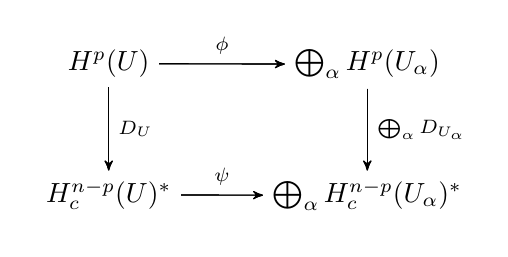
\begin{tikzpicture}
	\matrix (m) [matrix of math nodes, row sep=3em, column sep=3em]
	{  
		H^{p}(U) & \bigoplus_{\alpha} H^{p}(U_{\alpha})
		\\
		H^{n - p}_{c}(U)^{*} & \bigoplus_{\alpha}H^{n - p}_{c}(U_{\alpha})^{*}
		\\
	};
	{ [start chain] 
		\chainin (m-1-1);
		{ [start branch=A] \chainin (m-2-1)
			[join={node[right,labeled] {D_{U}}}];
		}
		\chainin (m-1-2) [join={node[above,labeled] {\phi} }];
		{ [start branch=A] \chainin (m-2-2)
			[join={node[right,labeled] { \bigoplus_{\alpha}D_{U_{\alpha}} }}];
		}
	}
	{ [start chain] 
		\chainin (m-2-1);
		\chainin (m-2-2) [join={node[above,labeled] {\psi}}];
	}
	\end{tikzpicture}
	\\
	e por hipótese $\{U_{\alpha} \subset M^{n}: \alpha \in J \}$ saõ subconjuntos abertos de $M$ são dois a dois disjuntos, então, pelo \textit{lema} anterior, temos os isomorfismos $\phi$ e $\psi$. Definindo $\bigoplus_{\alpha}D_{U_{\alpha}} : \bigoplus_{\alpha} \cohomologia{p}{U_{\alpha}} \to \bigoplus_{\alpha} \cohomologiacompacdual{n-p}{U_{\alpha}}$ tal que $\bigoplus_{\alpha}D_{U_{\alpha}} (\bigoplus_{\beta}[\omega_{\beta}]) = \bigoplus_{\alpha}D_{U_{\alpha}} ([\omega_{\alpha}])$, e como $D_{U_{\alpha}}$ é um isomorfismo para para $\alpha \in J$, então $\bigoplus_{\alpha}D_{U_{\alpha}}$ é um isomorfismo. Pela sequência de Mayer-Vietoris temos a comutatividade do diagrama expressa pela comutação dos seguintes morfismos $(\bigoplus_{\alpha}D_{U_{\alpha}}) \circ \phi = \psi \circ D_{U}$, e como $(\bigoplus_{\alpha}D_{U_{\alpha}}) \circ \phi$ é um isomorfismo pois é a composição de isomorfismos, então afirmar que $D_{U} = \psi^{-1} \circ (\bigoplus_{\alpha}D_{U_{\alpha}}) \circ \phi$, portanto é um isomorfismo pois é a composição de isomorfismos.
	
	Para 3) por hipótese $U \subseteq M$ é difeomorfo a $\real{n}$, logo é homeomorfo, e pelo \textit{corolário dos isomorfismos da dualidade do $\real{n}$}, temos que $D_{U}$ é um isomorfismo.
	
	$\blacksquare$
	
	\vspace{2mm}
	O próximos teorema é demasiadamente técnico e suas demonstrações estão fora do escopo pois não acrescentarão ao entendimento do conteúdo aqui exposto.
	
	\vspace{2mm}
	\textit{\textbf{Teorema (indução em conjuntos abertos): Seja $M^{n}$ uma n-variedade diferenciável e $\mathcal{V} = (V_{i})_{i \in I}$} uma cobertura de abertos de $M$. Suponha que $\mathcal{U}$ seja uma coleção de subconjuntos abertos de $M$ tais que:}
	\begin{enumerate}
		
		\item $\emptyset \in \mathcal{U}$,
		
		\item \textit{Qualquer aberto $U \subseteq V_{i}$ difeomorfo a $\real{n}$ esta em $\mathcal{U}$,}
		
		\item \textit{Se $U_{1}, U_{2}, U_{1}\cap U_{2} \subset \mathcal{U}$, então $U_{1} \cup U_{2} \subset \mathcal{U}$,}
		
		\item \textit{Se $(U_{k})_{k \in \mathbb{N}}$ é uma sequência de subconjuntos abertos de $\mathcal{U}$ dois a dois disjuntos, então $\bigcup_{k \in \mathbb{N}}U_{k} \subset \mathcal{U}$.}
	\end{enumerate}
	\textit{Nessa condições teremos que $M \subset \mathcal{U}$}.
	
	$\square$ A demonstração esta fora do escopo.
	
	$\blacksquare$
	
	\vspace{2mm}
	\textit{\textbf{Teorema (dualidade de Poincaré):} Seja $M^{n}$ uma n-variedade diferenciável e orientável, então temos o isomorfismo}
	$$
	D_{M}:\cohomologia{p}{M} \to \cohomologiacompacdual{n-p}{M}, \; 0\leq p \leq n.
	$$
	
	$\square$ Seja $\mathcal{U} = \{U \subseteq M: D_{U}\; \textit{é isomorfismo} \}$ uma coleção de abertos, e $\mathcal{V} = (V_{i})_{i \in I} = (M)$ uma cobertura trivial consistindo apenas de $M$. Essa coleção é não-vazia pois o \textit{teorema da existência da dualidade de Poincaré} nos garante essa condição. Vejamos que a família $\mathcal{U}$ cumpre as condições do \textit{teorema de indução de conjuntos abertos} pois: 1) vejamos que $\cohomologia{p}{\emptyset} = 0$ para $0\leq p \leq n$, logo $D_{\emptyset}$ é o isomorfismo trivial, portanto $\emptyset \in \mathcal{U}$; 2) pelo \textit{corolário das dualidades locais} se $U \subseteq V_{i} = M$ for difeomorfo a $\real{n}$, então $D_{U}$ é um isomorfismo, logo $U \in \mathcal{U}$; 3) dados $U_{1}, U_{2}, U_{1}\cap U_{2} \in \mathcal{U}$, então $D_{U_{1}}, D_{U_{2}}, D_{U_{1} \cap U_{2}}$ são isomorfismo, logo pelo \textit{corolário das dualidades locais} $D_{U_{1} \cup U_{2}}$ é um isomorfismo, e como $U_{1} \cup U_{2}$ é uma união finita de abertos, portanto aberto, então $U_{1} \cup U_{2} \in \mathcal{U}$; 4) seja $(U_{k})_{k \in \mathbb{N}}$ uma família de elementos de $\mathcal{U}$ dois a dois disjuntos, consequementemente $D_{k}$ é um isomorfismo para cada $k \in \mathbb{N}$, então pelo \textit{corolário das dualidades locais} temos que $D_{U}$ é um isomorfismo para $U = \bigcup_{k}U_{k}$, e como $U$ é uma união arbitrária de abertos, logo aberto, então $U = \bigcup_{k}U_{k} \in \mathcal{U}$. Cumpridas todas as condições, temos que, pelo \textit{teorema de indução em conjuntos abertos} que $M \in \mathcal{U}$, o que implica que $D_{M}$ é um isomorfismo, como desejávamos.
	
	$\blacksquare$
\end{document}